\chapter{PENGUJIAN DAN ANALISIS}
\label{chap:pengujiananalisis}

% Ubah bagian-bagian berikut dengan isi dari pengujian dan analisis

Pada bab ini akan dipaparkan mengenai hasil pengujian dan pembahasan dari penelitian yang telah dipaparkan pada metodologi. Dipaparkan juga mengenai skenario pengujian yang dilakukan. 

\section{Skenario Pengujian}
Pengujian dilakukan untuk mengetahui performa model dalam melakukan klasifikasi. Skenario pengujian yang akan dilakukan adalah sebagai berikut:
\begin{enumerate}
    \item Pengujian Performa Model %\emph{Confusion Matrix}
    \item Pengujian Performa Model dengan Variasi Jarak Kamera
    \item Pengujian Performa Model dengan Variasi Pencahayaan
    \item Pengujian Kecepatan FPS 
    \item Pengujian Waktu Respons Kontrol Kursi Roda
    \item Pengujian kestabilan Performa Kursi Roda 
\end{enumerate}

\section{Pengujian Performa Model}

Dalam pembuatan model \emph{ConvolutionalNeuralNetwork} (CNN) yang akan digunakan, dilakukan pengelompokkan data citra kedalam lima kelas yang kemudian akan di\emph{training}. Lima kelas tersebut adalah Kanan, Kiri, Maju, Mundur, dan \emph{Stop}. Total data citra yang dijadikan sebagai dataset berjumlah 2450. Data tersebut kemudian dibagi menjadi dua buah dataset, yaitu dataset \emph{training} dan dataset \emph{validation} dengan rasio pembagian 80:20, sehingga data yang digunakan berjumlah 392 data \emph{training} dan 98 data \emph{validation} untuk tiap kelasnya. Pembagian dataset yang dilakukan telah divisualisasikan pada diagram Gambar \ref{fig:pembagiandataset}. Pada skenario pengujian ini terdapat dua buah model yang memiliki perbedaan pada jumlah filet di layer yang digunakan. Pengujian ini dilakukan untuk mendapatkan model yang memiliki performa terbaik dalam melakukan klasifikasi. Model yang memiliki performa terbaik akan digunakan untuk pengujian selanjutnya.

\begin{figure}[H]
  \centering
  % Nama dari file gambar yang diinputkan
  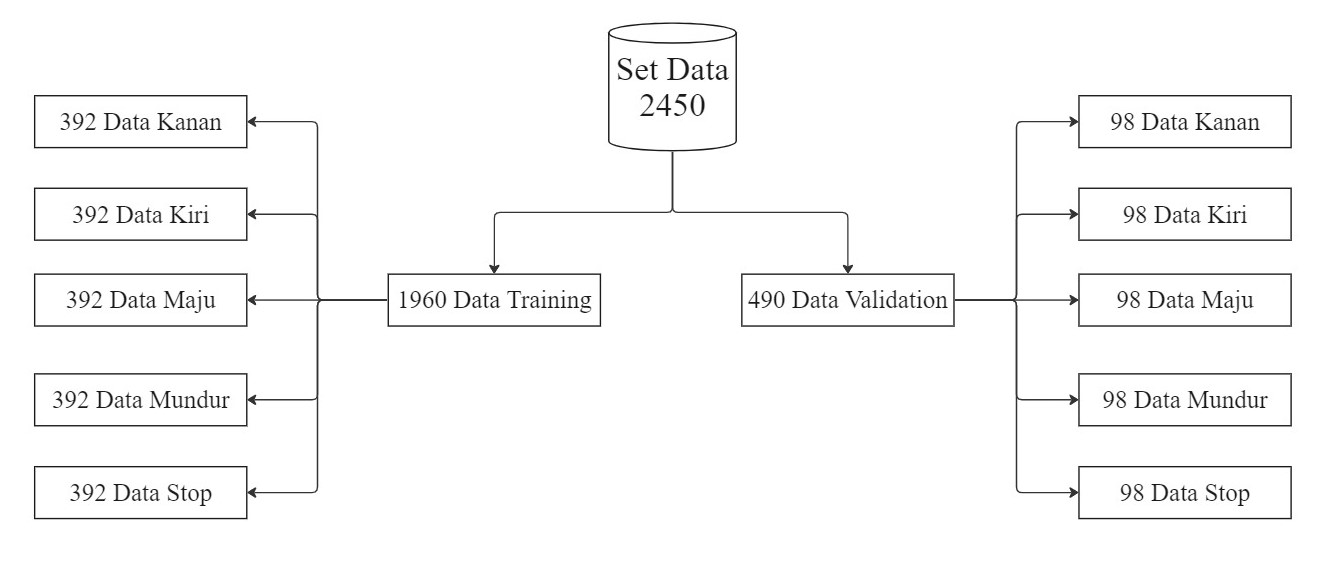
\includegraphics[scale=0.5]{gambar/pembagiandataset.jpg}
  % Keterangan gambar yang diinputkan
  \caption{Diagram Pembagian Dataset}
  % Label referensi dari gambar yang diinputkan
  \label{fig:pembagiandataset}
\end{figure}


\subsection{Pengujian Model Pertama}
Model pertama memiliki 64 filter pada layer pertama, 256 unit pada layer ketiga, dan 512 unit pada dense layer pertama. Berdasarkan grafik yang didapat setelah dilakukan \emph{training}, model ini memiliki \emph{training accuracy} sebesar 100\% dan \emph{validation accuracy} sebesar 99.80\% seperti pada Gambar \Ref{fig:AccuracyHasilPelatihanModel}. Model ini juga memiliki \emph{training loss} sebesar 0.0307 dan \emph{validation loss} sebesar 0.0104 yang dapat dilihat pada Gambar \Ref{fig:LossHasilPelatihanModel}. \emph{Training loss} dan \emph{validation loss} yang didapat sangatlah kecil yang berarti error yang didapat sangatlah kecil yang berarti pendeteksian model sangatlah efisien.

\begin{figure}[H]
  \centering
  % Nama dari file gambar yang diinputkan
  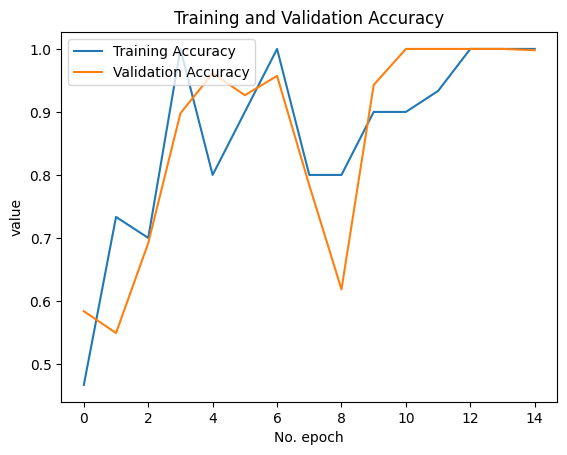
\includegraphics[scale=0.7]{gambar/normal accuracy.png}
  % Keterangan gambar yang diinputkan
  \caption{Accuracy Hasil Pelatihan Model}
  % Label referensi dari gambar yang diinputkan
  \label{fig:AccuracyHasilPelatihanModel}
\end{figure}


\begin{figure}[H]
  \centering
  % Nama dari file gambar yang diinputkan
  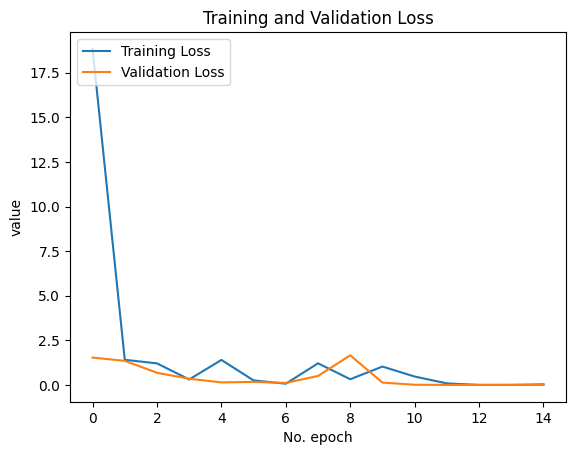
\includegraphics[scale=0.7] {gambar/normal loss.png}
  % Keterangan gambar yang diinputkan
  \caption{Model Loss Hasil Pelatihan Model}
  % Label referensi dari gambar yang diinputkan
  \label{fig:LossHasilPelatihanModel}
\end{figure}

\begin{figure} [H] \centering
  % Nama dari file gambar yang diinputkan
  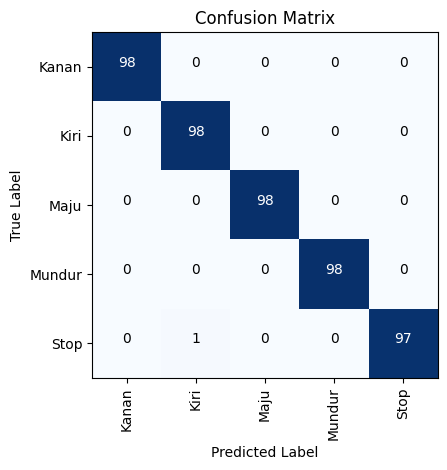
\includegraphics[scale=0.8]{gambar/normal confusion.png}
  % Keterangan gambar yang diinputkan
  \caption{Confusion Matrix Hasil Pelatihan Model Pertama}
  % Label referensi dari gambar yang diinputkan
  \label{fig:ConfusionMatrixHasilPelatihanModel}
\end{figure}

Dalam pengujian model CNN yang telah dibuat terhadap data validasi, dengan menggunakan perhitungan \emph{confusion matrix}, didapatkan hasil klasifikasi seperti yang telah divisualisasikan pada Gambar \ref{fig:ConfusionMatrixHasilPelatihanModel}. Dari Gambar tersebut, dapat dilihat bahwa dari 490 data pada model yang diujikan terhadap data citra validasi, terdapat 1 data citra yang hasil prediksinya tidak sesuai dengan data aktual yang diujikan. Satu data citra tersebut merupakan data citra dari kelas \emph{stop} yang 1 data terdeketsi sebagai data citra kelas kiri. Persentase keberhasilan pada kelas \emph{stop} adalah sekitar 98,98\% dengan jumlah 97 data dan persentase ketidakberhasilannya adalah sekitar 1,02\% dengan jumlah 1 data. Pada Tabel \ref{tb:Hasil Klasifikasi Model Pertama} dapat dilihat terdapat 1 data kelas \emph{stop} yang terdeteksi sebagai \emph{false negative} dan 97 data yang terdeteksi sebagai \emph{true positive}. Selain itu, dapat dilihat juga terdapat 1 data kelas kiri yang terdeteksi sebagai \emph{false positive} dan 391 data yang terdeteksi sebagai \emph{true negative}.


\begin{table}[H]
  \centering
  \caption{Hasil Klasifikasi Model Pertama}
  \label{tb:Hasil Klasifikasi Model Pertama}
  \begin{tabular}{|c|c|c|c|c|}
  \hline
  \rowcolor[HTML]{9B9B9B} 
  \cellcolor[HTML]{9B9B9B} & TP & TN  & FP & FN \\ \hline
  Kanan                    & 98 & 392 & 0  & 0  \\ \hline
  Kiri                     & 98 & 391 & 1  & 0  \\ \hline
  Maju                     & 98 & 392 & 0  & 0  \\ \hline
  Mundur                   & 98 & 392 & 0  & 0  \\ \hline
  Stop                     & 97 & 392 & 0  & 1  \\ \hline
  \end{tabular}
  \end{table}

  Pada Tabel \ref{tb:Hasil Validasi Nilai Model Pertama} dapat dilihat bahwa nilai \emph{accuracy} pada kiri adalah sebesar 0.998 dan nilai \emph{precision}nya 0.9899. Hal ini menyebabkan kelas kiri memiliki \emph{F1-Score} sebesar 0.9949. Sedangkan pada kelas \emph{stop}, nilai \emph{accuracy}nya adalah 0.998 dan nilai \emph{recall}nya 0.9898. Hal ini menyebabkan kelas \emph{stop} memiliki \emph{F1-Score} sebesar 0.9949. Pada kelas kanan, maju, dan mundur memiliki nilai \emph{accuracy}, \emph{precision}, \emph{recall}, dan \emph{F1-Score} sebesar 1.0000.

  \begin{table}[H]
    \centering
    \caption{Hasil Validasi Nilai Model Pertama}
    \label{tb:Hasil Validasi Nilai Model Pertama}
  \begin{tabular}{|c|c|c|c|c|}
    \hline
    \rowcolor[HTML]{9B9B9B} 
    \cellcolor[HTML]{9B9B9B} & Accuracy & Precision & Recall & F1-Score \\ \hline
    Kanan                    & 1.0000    & 1.0000    & 1.0000 & 1.0000   \\ \hline
    Kiri                     & 0.9980    & 0.9899    & 1.0000 & 0.9949   \\ \hline
    Maju                     & 1.0000    & 1.0000    & 1.0000 & 1.0000   \\ \hline
    Mundur                   & 1.0000    & 1.0000    & 1.0000 & 1.0000   \\ \hline
    Stop                     & 0.9980    & 1.0000    & 0.9898 & 0.9949   \\ \hline
    \end{tabular}
    \end{table}


Pada pengujian ini, dilakukan 480 kali pendeteksian yang mana kemudian akan dihitung perbandingan terdeteksi dan tidaknya pada tiap model yang diujikan. Hasil yang didapatkan dari pengujian ini dapat dilihat pada Tabel \ref{tb:Hasil Pengujian Keterdeteksian Model Pertama}. Dari hasil pengujian ini, dapat dilihat bahwa model pertama memiliki persentase keberhasilan sebesar 98,125\% dan persentase ketidakberhasilan sebesar 1,875\%. Hal ini menunjukkan bahwa model pertama memiliki performa yang sangat baik dalam melakukan klasifikasi secara \emph{real-time}.

    \begin{longtable}{|c|c|}
      \caption{Hasil Pengujian Keterdeteksian Model Pertama}
      \label{tb:Hasil Pengujian Keterdeteksian Model Pertama}   \\
      \hline
      \cellcolor[HTML]{C0C0C0}
      \textbf{Jumlah Keberhasilan:} & 471\\
      \hline
      \cellcolor[HTML]{C0C0C0}
      \textbf{Jumlah Ketidakberhasilan:} & 9\\
      \hline
      \cellcolor[HTML]{C0C0C0}
      \textbf{Persentasi Keberhasilan:} & 98,125\% \\
      \hline
      \cellcolor[HTML]{C0C0C0}
      \textbf{Persentasi Ketidakberhasilan:} & 1,875\% \\
      \hline
      \end{longtable}
    
\subsection{Pengujian Model Kedua}
Model kedua  memiliki 64 filter pada layer pertama, 128 unit pada layer ketiga, dan 256 unit pada dense layer pertama. Berdasarkan grafik yang didapat setelah dilakukan \emph{training}, model ini memiliki \emph{training accuracy} sebesar 100\% dan \emph{validation accuracy} sebesar 100.00\% seperti pada Gambar \Ref{fig:AccuracyHasilPelatihanModelKedua}. Model ini juga memiliki \emph{training loss} sebesar 0.0005 dan \emph{validation loss} sebesar 0.0020 yang dapat dilihat pada Gambar \Ref{fig:LossHasilPelatihanModelKedua}. \emph{Training loss} dan \emph{validation loss} yang didapat sangatlah kecil yang berarti error yang didapat sangatlah kecil yang berarti pendeteksian model sangatlah efisien.

\begin{figure}[H]
  \centering
  % Nama dari file gambar yang diinputkan
  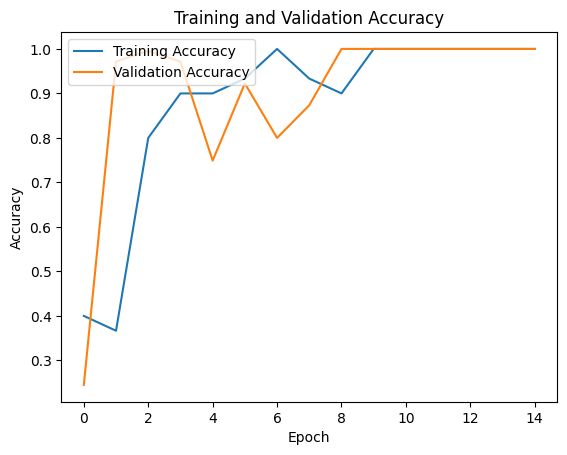
\includegraphics[scale=0.7]{gambar/accuracytdk.png}
  % Keterangan gambar yang diinputkan
  \caption{Accuracy Hasil Pelatihan Model Kedua}
  % Label referensi dari gambar yang diinputkan
  \label{fig:AccuracyHasilPelatihanModelKedua}
\end{figure}

\begin{figure}[H]
  \centering
  % Nama dari file gambar yang diinputkan
  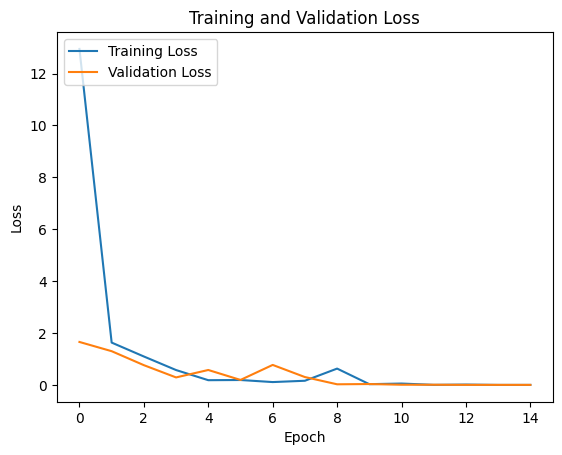
\includegraphics[scale=0.7]{gambar/losstdk.png}
  % Keterangan gambar yang diinputkan
  \caption{Model Loss Hasil Pelatihan Model Kedua}
  % Label referensi dari gambar yang diinputkan
  \label{fig:LossHasilPelatihanModelKedua}
\end{figure}

\begin{figure} [H] \centering
  % Nama dari file gambar yang diinputkan
  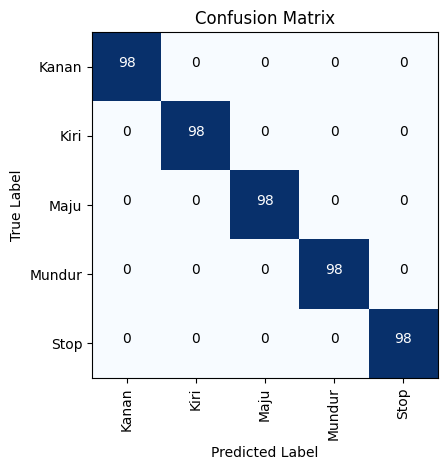
\includegraphics[scale=0.8]{gambar/connfusiontdk.png}
  % Keterangan gambar yang diinputkan
  \caption{Confusion Matrix Hasil Pelatihan Model Kedua}
  % Label referensi dari gambar yang diinputkan
  \label{fig:ConfusionMatrixHasilPelatihanModelKedua}
\end{figure}

Dalam pengujian model CNN yang telah dibuat terhadap data validasi, dengan menggunakan perhitungan \emph{confusion matrix}, didapatkan hasil klasifikasi seperti yang telah divisualisasikan pada Gambar \ref{fig:ConfusionMatrixHasilPelatihanModelKedua}. Dari Gambar tersebut, dapat dilihat bahwa dari 490 data pada model yang diujikan terhadap data citra validasi, tidak terdapat data citra yang hasil prediksinya tidak sesuai dengan data aktual yang diujikan. Hal ini membuat persentase keberhasilan pada kelas kiri, kanan, maju, dan mundur adalah sebesar 100\% dan persentase ketidakberhasilannya adalah sebesar 0\%. Pada Tabel \ref{tb:Hasil Klasifikasi Model Kedua} dapat dilihat tidak terdapat data yang terdeteksi sebagai \emph{false negative} dan \emph{false positive} pada setiap kelasnya.

\begin{table}[H]
  \centering
  \caption{Hasil Klasifikasi Model Kedua}
  \label{tb:Hasil Klasifikasi Model Kedua}
  \begin{tabular}{|c|c|c|c|c|}
    \hline
    \rowcolor[HTML]{9B9B9B} 
    \cellcolor[HTML]{9B9B9B} & TP & TN  & FP & FN \\ \hline
    Kanan                    & 98 & 392 & 0  & 0  \\ \hline
    Kiri                     & 98 & 392 & 0  & 0  \\ \hline
    Maju                     & 98 & 392 & 0  & 0  \\ \hline
    Mundur                   & 98 & 392 & 0  & 0  \\ \hline
    Stop                     & 98 & 392 & 0  & 0  \\ \hline
    \end{tabular}
    \end{table}


  Pada Tabel \ref{tb:Hasil Validasi Nilai Model Kedua} pada semua kelas, nilai \emph{accuracy}, \emph{precision}, dan \emph{recall} bernilai 1.0000. Hal ini memebuat semua kelas memiliki nilai \emph{F1-Score} sebesar 1.0000. Hal ini menunjukkan bahwa model kedua memiliki performa yang sangat baik dalam melakukan klasifikasi.  

  \begin{table}[H]
    \centering
    \caption{Hasil Validasi Nilai Model Kedua}
    \label{tb:Hasil Validasi Nilai Model Kedua}
    \begin{tabular}{|c|c|c|c|c|}
      \hline
      \rowcolor[HTML]{9B9B9B} 
      \cellcolor[HTML]{9B9B9B} & Accuracy & Precision & Recall & F1-Score \\ \hline
      Kanan                    & 1.0000   & 1.0000    & 1.0000 & 1.0000   \\ \hline
      Kiri                     & 1.0000   & 1.0000    & 1.0000 & 1.0000   \\ \hline
      Maju                     & 1.0000   & 1.0000    & 1.0000 & 1.0000   \\ \hline
      Mundur                   & 1.0000   & 1.0000    & 1.0000 & 1.0000   \\ \hline
      Stop                     & 1.0000   & 1.0000    & 1.0000 & 1.0000   \\ \hline
      \end{tabular}
      \end{table}

Pada pengujian ini, dilakukan 480 kali pendeteksian yang mana kemudian akan dihitung perbandingan terdeteksi dan tidaknya pada tiap model yang diujikan. Hasil yang didapatkan dari pengujian ini dapat dilihat pada Tabel \ref{tb:Hasil Pengujian Keterdeteksian Model Kedua}. Dari hasil pengujian ini, dapat dilihat bahwa model kedua memiliki persentase keberhasilan sebesar 69,375\% dan persentase ketidakberhasilan sebesar 30,625\%. Hal ini menunjukkan bahwa performa model kedua dalam melakukan klasifikasi secara \emph{real-time} tidak sebaik model pertama. Karena model pertama memiliki performa yang lebih baik dibandingkan model kedua, maka model pertama yang akan digunakan untuk pengujian selanjutnya.

      \begin{longtable}{|c|c|}
        \caption{Hasil Pengujian Keterdeteksian Model Kedua}
        \label{tb:Hasil Pengujian Keterdeteksian Model Kedua}   \\
        \hline
        \cellcolor[HTML]{C0C0C0}
        \textbf{Jumlah Keberhasilan:} & 333\\
        \hline
        \cellcolor[HTML]{C0C0C0}
        \textbf{Jumlah Ketidakberhasilan:} & 147\\
        \hline
        \cellcolor[HTML]{C0C0C0}
        \textbf{Persentasi Keberhasilan:} & 69,375\% \\
        \hline
        \cellcolor[HTML]{C0C0C0}
        \textbf{Persentasi Ketidakberhasilan:} & 30,625\% \\
        \hline
        \end{longtable}


\section{Pengujian Performa Model dengan Variasi Jarak Kamera}
Pada skenario pengujian ini, digunakan variasi jarak dari citra wajah ke \emph{webcam} yang digunakan sebagai variabel bebasnya. Digunakan jarak 50 sentimeter, 75 sentimeter, dan 100 sentimeter untuk tiap-tiap pengujian. Perbandingan gambar dataset dapat dilihat pada Tabel \ref{tab:Variasi Jarak Kamera}.Variabel terikat yang akan didapatkan dari pengujian ini adalah berupa nilai dari \emph{accuracy}, \emph{loss}, dan \emph{confusion matrix}. Pada setiap dataset akan dilakukan \emph{training} sebanyak 15 \emph{epoch} dengan ukuran citra wajah yang telah disamaratakan sebesar 140 x 140. Hasil yang didapatkan dari pengujian performa model dengan variasi jarak kamera yang telah dilakukan menunjukkan bahwa model yang memiliki akurasi pendeteksian yang paling baik adalah model yag diambil dengan jarak antara wajah dan kamera sejauh 50 sentimeter. Untuk pembahasan lebih detailnya mengenai penelitian ini dapat dilihat dari subbab masing-masing jarak dibawah ini.

\begin{table}[H]
  \centering
  \begin{tabular}{|c|c|}
  \hline
  \textbf{Jarak Kamera} & \textbf{Contoh Dataset} \\ \hline
  50 & 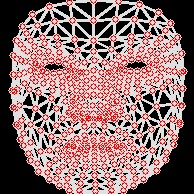
\includegraphics[width=0.4\textwidth]{gambar/50 stop.jpg} \\ \hline
  75 & 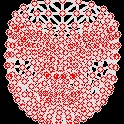
\includegraphics[width=0.4\textwidth]{gambar/75 stop.jpg} \\ \hline
  100 & 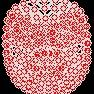
\includegraphics[width=0.4\textwidth]{gambar/100 stop.jpg} \\ \hline
  \end{tabular}
  \caption{Variasi Jarak Kamera}
  \label{tab:Variasi Jarak Kamera}
  \end{table}

\subsection{Pengujian jarak 50 sentimeter}
Pada bagian pengujian ini, citra wajah yang diambil sebagai dataset diambil dari jarak 50 sentimeter dari \emph{webcam} yang digunakan. Diambil sebanyak 490 data citra wajah untuk setiap kelasnya yang berarti terdapat total 2450 data citra dari kelima kelas yang ada. Kemudian, dataset tersebut dibagi menjada dataset \emph{training} dan dataset \emph{validation} dengan rasio perbandingan 80 : 20 sehingga didapatkan 392 data citra wajah yang dijadikan sebagai dataset \emph{training} dan 98 data citra wajah sebagai dataset \emph{validation} untuk setiap kelasnya.

\begin{figure}[H]
  \centering
  \begin{subfigure}{0.3\textwidth}
      \centering
      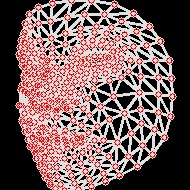
\includegraphics[width=\linewidth]{gambar/50 kanan.jpg}
      \caption{Citra kelas kanan}
      \label{fig:image1}
  \end{subfigure}
  \hfill
  \begin{subfigure}{0.3\textwidth}
      \centering
      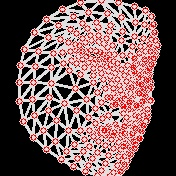
\includegraphics[width=\linewidth]{gambar/50 kiri.jpg}
      \caption{Citra kelas kiri}
      \label{fig:image2}
  \end{subfigure}
  \hfill
  \begin{subfigure}{0.3\textwidth}
      \centering
      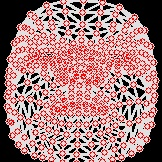
\includegraphics[width=\linewidth]{gambar/50 maju.jpg}
      \caption{Citra kelas maju}
      \label{fig:image3}
  \end{subfigure}
  
  \begin{subfigure}{0.3\textwidth}
      \centering
      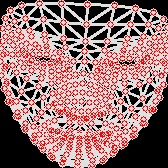
\includegraphics[width=\linewidth]{gambar/50 mundur.jpg}
      \caption{Citra kelas mundur}
      \label{fig:image4}
  \end{subfigure}
  \hfill
  \begin{subfigure}{0.3\textwidth}
      \centering
      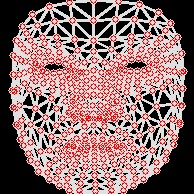
\includegraphics[width=\linewidth]{gambar/50 stop.jpg}
      \caption{Citra kelas \emph{stop}}
      \label{fig:image5}
  \end{subfigure}
  \caption{Dataset Jarak 50 sentimeter}
  \label{fig:15lux}
\end{figure}


Berdasarkan grafik yang didapat setelah dilakukan \emph{training}, model yag diambil dari jarak 50 sentimeter ini memiliki \emph{training accuracy} sebesar 100\% dan \emph{validation accuracy} sebesar 97.76\% seperti pada Gambar \ref{fig:AccuracyHasilPelatihanJarak50cm}. Hal ini menunjukkan bahwa prediksi terhadap model pada dataset training semuanya akurat dan pada dataset validation juga memiliki akurasi yang tinggi meskipun tidak semuanya akurat. Model ini juga memiliki \emph{training loss} sebesar 0.0001 dan \emph{validation loss} sebesar 0.0960 yang dapat dilihat pada Gambar \ref{fig:LossHasilPelatihanJarak50cm}. \emph{Training loss} dan \emph{validation loss} yang didapat sangatlah kecil yang berarti error yang didapat sangatlah kecil yang berarti pendeteksian model sangatlah efisien. Selain itu, dapat dilihat juga pada grafik bahwa \emph{training} yang dilakukan belum selesai di 15 \emph{epoch}.  


\begin{figure} [H] \centering
  % Nama dari file gambar yang diinputkan
  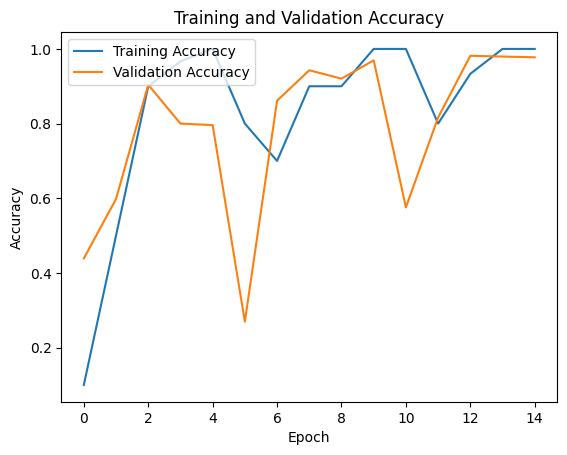
\includegraphics[scale=0.7]{gambar/50accuracy.png}
  % Keterangan gambar yang diinputkan
  \caption{Accuracy Hasil Pelatihan Jarak 50cm}
  % Label referensi dari gambar yang diinputkan
  \label{fig:AccuracyHasilPelatihanJarak50cm}
\end{figure}

\begin{figure} [H] \centering
  % Nama dari file gambar yang diinputkan
  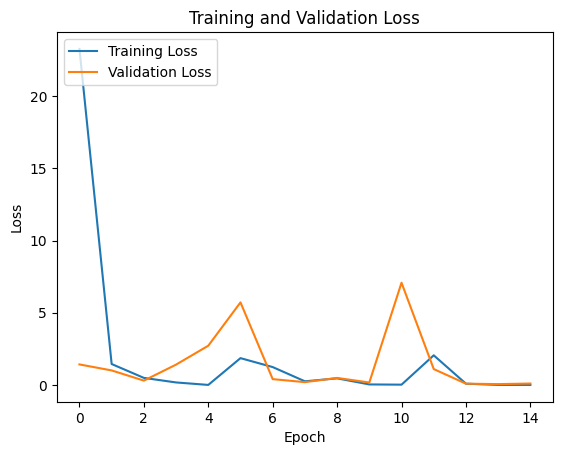
\includegraphics[scale=0.7]{gambar/50loss.png}
  % Keterangan gambar yang diinputkan
  \caption{Loss Hasil Pelatihan Jarak 50cm}
  % Label referensi dari gambar yang diinputkan
  \label{fig:LossHasilPelatihanJarak50cm}
\end{figure}

Dalam pengujian model CNN yang telah dibuat terhadap data validasi dan diambil dengan jarak 50 sentimeter, dengan menggunakan perhitungan \emph{confusion matrix}, didapatkan hasil klasifikasi seperti yang telah divisualisasikan pada Gambar \ref{fig:ConfusionMatrixHasilPelatihanJarak50cm}. Dari Gambar \ref{fig:ConfusionMatrixHasilPelatihanJarak50cm}, dapat dilihat bahwa dari 490 data pada model yang diujikan terhadap data citra validasi, terdapat 11 data citra yang hasil prediksinya tidak sesuai dengan data aktual yang diujikan. Sebelas data citra tersebut merupakan data citra dari kelas kiri yang 4 data terdeketsi sebagai data citra kelas kanan dan 7 data citra terdeteksi sebagai kelas \emph{stop}. Persentase keberhasilan pada kelas kiri adalah sekitar 88,78\% dengan jumlah 87 data dan persentase ketidakberhasilannya adalah sekitar 11,22\% dengan jumlah 11 data. Dengan detail persentase ketidakberhasilan 7,14\% terdeketsi sebagai kelas \emph{stop} dan 4,08\% terdeteksi sebagai citra kelas kanan. Pada Tabel \ref{tb:Hasil Klasifikasi Jarak 50cm} dapat dilihat terdapat 1 data kelas kanan yang terdeteksi sebagai \emph{false negative} dan 97 data yang terdeteksi sebagai \emph{true positive}. Selain itu, dapat dilihat juga terdapat 1 data kelas \emph{stop} yang terdeteksi sebagai \emph{false positive} dan 391 data yang terdeteksi sebagai \emph{true negative}.

\begin{figure} [H] \centering
  % Nama dari file gambar yang diinputkan
  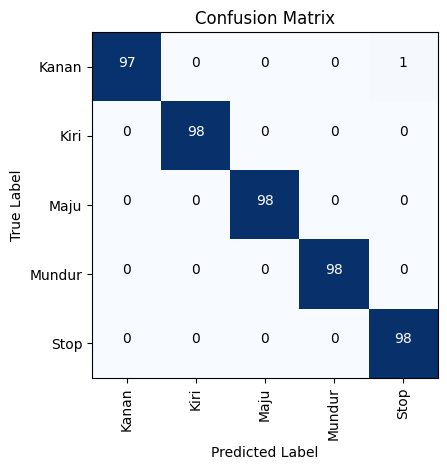
\includegraphics[scale=0.8]{gambar/50confusion.png}
  % Keterangan gambar yang diinputkan
  \caption{Confusion Matrix Hasil Pelatihan Jarak 50cm}
  % Label referensi dari gambar yang diinputkan
  \label{fig:ConfusionMatrixHasilPelatihanJarak50cm}
\end{figure}


\begin{table}[H]
  \centering
  \caption{Hasil Klasifikasi Model Jarak 50cm}
  \label{tb:Hasil Klasifikasi Jarak 50cm}
\begin{tabular}{|c|c|c|c|c|}
  \hline
  \rowcolor[HTML]{C0C0C0} 
  \cellcolor[HTML]{C0C0C0} & TP & TN  & FP & FN \\ \hline
  Kanan                    & 97 & 392 & 0  & 1  \\ \hline
  Kiri                     & 98 & 392 & 0  & 0  \\ \hline
  Maju                     & 98 & 392 & 0  & 0  \\ \hline
  Mundur                   & 98 & 392 & 0  & 0  \\ \hline
  Stop                     & 98 & 391 & 1  & 0  \\ \hline
  \end{tabular}
  \end{table}

Pada Tabel \ref{tb:Hasil Validasi Nilai Model Jarak 50cm} dapat dilihat bahwa nilai \emph{accuracy} pada kelas kanan adalah sebesar 0.9898 dan nilai \emph{recall}nya 0.9898. Hal ini menyebabkan kelas kanan memiliki \emph{F1-Score} sebesar 0.9949. Sedangkan pada kelas \emph{stop}, nilai \emph{accuracy}nya adalah 0.998 dan nilai \emph{precision}nya 0.9899. Hal ini menyebabkan kelas kiri memiliki \emph{F1-Score} sebesar 0.9949. Pada kelas kiri, maju, dan mundur memiliki nilai \emph{accuracy}, \emph{precision}, \emph{recall}, dan \emph{F1-Score} sebesar 1.0000.

\begin{table}[H]
  \centering
  \caption{Hasil Validasi Nilai Model Jarak 50cm}
  \label{tb:Hasil Validasi Nilai Model Jarak 50cm}
  \begin{tabular}{|c|c|c|c|c|}
    \hline
    \rowcolor[HTML]{C0C0C0} 
    \cellcolor[HTML]{C0C0C0} & Accuracy & Precision & Recall & F1-Score \\ \hline
    Kanan                    & 0.998    & 1.0000    & 0.9898 & 0.9949   \\ \hline
    Kiri                     & 1.000    & 1.0000    & 1.0000 & 1.0000   \\ \hline
    Maju                     & 1.000    & 1.0000    & 1.0000 & 1.0000   \\ \hline
    Mundur                   & 1.000    & 1.0000    & 1.0000 & 1.0000   \\ \hline
    Stop                     & 0.998    & 0.9899    & 1.0000 & 0.9949   \\ \hline
    \end{tabular}
    \end{table}

\subsection{Pengujian jarak 75 sentimeter}
Pada bagian pengujian ini, citra wajah yang diambil sebagai dataset diambil dari jarak 75 sentimeter dari \emph{webcam} yang digunakan. Diambil sebanyak 490 data citra wajah untuk setiap kelasnya yang berarti terdapat total 2450 data citra dari kelima kelas yang ada. Kemudian, dataset tersebut dibagi menjada dataset \emph{training} dan dataset \emph{validation} dengan rasio perbandingan 80 : 20 sehingga didapatkan 392 data citra wajah yang dijadikan sebagai dataset \emph{training} dan 98 data citra wajah sebagai dataset \emph{validation} untuk setiap kelasnya.

\begin{figure}[H]
  \centering
  \begin{subfigure}{0.3\textwidth}
      \centering
      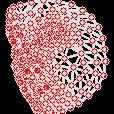
\includegraphics[width=\linewidth]{gambar/75 kanan.jpg}
      \caption{Citra kelas kanan}
      \label{fig:image1}
  \end{subfigure}
  \hfill
  \begin{subfigure}{0.3\textwidth}
      \centering
      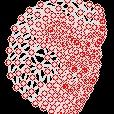
\includegraphics[width=\linewidth]{gambar/75 kiri.jpg}
      \caption{Citra kelas kiri}
      \label{fig:image2}
  \end{subfigure}
  \hfill
  \begin{subfigure}{0.3\textwidth}
      \centering
      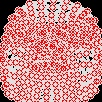
\includegraphics[width=\linewidth]{gambar/75 maju.jpg}
      \caption{Citra kelas maju}
      \label{fig:image3}
  \end{subfigure}
  
  \begin{subfigure}{0.3\textwidth}
      \centering
      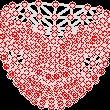
\includegraphics[width=\linewidth]{gambar/75 mundur.jpg}
      \caption{Citra kelas mundur}
      \label{fig:image4}
  \end{subfigure}
  \hfill
  \begin{subfigure}{0.3\textwidth}
      \centering
      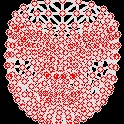
\includegraphics[width=\linewidth]{gambar/75 stop.jpg}
      \caption{Citra kelas \emph{stop}}
      \label{fig:image5}
  \end{subfigure}
  \caption{Dataset Jarak 75 sentimeter}
  \label{fig:15lux}
\end{figure}


Berdasarkan grafik yang didapat setelah dilakukan \emph{training}, model yag diambil dari jarak 75 sentimeter ini memiliki \emph{training accuracy} sebesar 90\% dan \emph{validation accuracy} sebesar 99.59\% seperti pada Gambar \ref{fig:AccuracyHasilPelatihanJarak75cm}. Model ini juga memiliki \emph{training loss} sebesar 0.0994 dan \emph{validation loss} sebesar 0.0103 yang dapat dilihat pada Gambar \ref{fig:LossHasilPelatihanJarak75cm}. Selain itu, dapat dilihat juga pada grafik bahwa \emph{training} yang dilakukan belum selesai di 15 \emph{epoch}.  

\begin{figure} [H] \centering
  % Nama dari file gambar yang diinputkan
  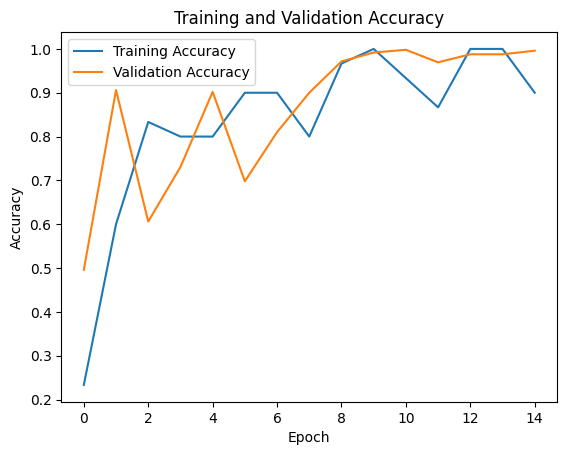
\includegraphics[scale=0.7]{gambar/75accuracy.png}
  % Keterangan gambar yang diinputkan
  \caption{Accuracy Hasil Pelatihan Jarak 75cm}
  % Label referensi dari gambar yang diinputkan
  \label{fig:AccuracyHasilPelatihanJarak75cm}
\end{figure}

\begin{figure} [H] \centering
  % Nama dari file gambar yang diinputkan
  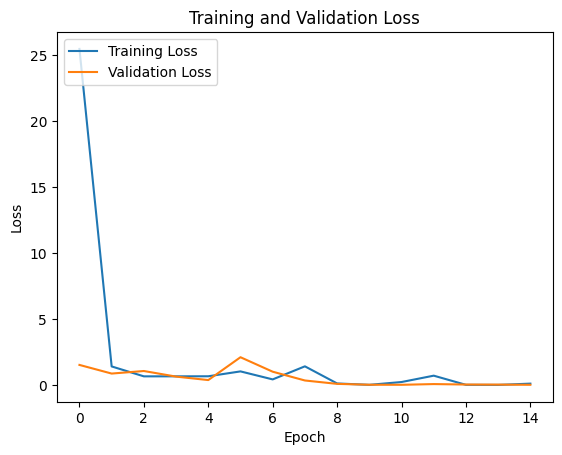
\includegraphics[scale=0.7]{gambar/75loss.png}
  % Keterangan gambar yang diinputkan
  \caption{Loss Hasil Pelatihan Jarak 75cm}
  % Label referensi dari gambar yang diinputkan
  \label{fig:LossHasilPelatihanJarak75cm}
\end{figure}

Dalam pengujian model CNN yang telah dibuat terhadap data validasi dan diambil dengan jarak 75 sentimeter, dengan menggunakan perhitungan \emph{confusion matrix}, didapatkan hasil klasifikasi seperti yang telah divisualisasikan pada Gambar \ref{fig:ConfusionMatrixHasilPelatihanJarak75cm}. Dari Gambar \ref{fig:ConfusionMatrixHasilPelatihanJarak75cm}, dapat dilihat bahwa dari 490 data pada model yang diujikan terhadap data citra validasi, terdapat 2 data citra yang hasil prediksinya tidak sesuai dengan data aktual yang diujikan. Dua data citra tersebut merupakan data citra dari kelas kiri yang terdeteksi sebagai data citra dari kelas \emph{stop}. Persentase keberhasilan pada kelas kiri adalah sekitar 97,96\% dengan jumlah 96 data dan persentase ketidakberhasilannya adalah sekitar 2,04\% dengan jumlah 2 data. Pada Tabel \ref{tb:Hasil Klasifikasi Jarak 75cm} dapat dilihat terdapat 2 data kelas kiri yang terdeteksi sebagai \emph{false negative} dan 96 data yang terdeteksi sebagai \emph{true positive}. Selain itu, dapat dilihat juga terdapat 2 data kelas \emph{stop} yang terdeteksi sebagai \emph{false positive} dan 390 data yang terdeteksi sebagai \emph{true negative}.

\begin{figure} [H] \centering
  % Nama dari file gambar yang diinputkan
  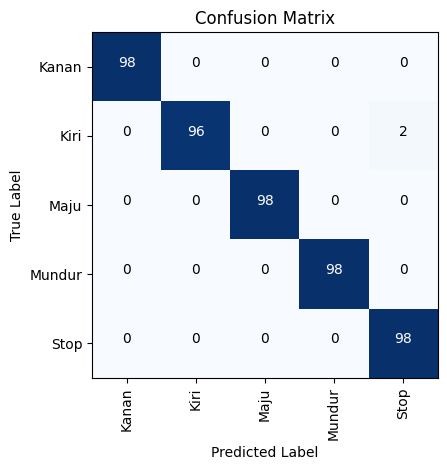
\includegraphics[scale=0.8]{gambar/75confusion.png}
  % Keterangan gambar yang diinputkan
  \caption{Confusion Matrix Hasil Pelatihan Jarak 75cm}
  % Label referensi dari gambar yang diinputkan
  \label{fig:ConfusionMatrixHasilPelatihanJarak75cm}
\end{figure}



\begin{table}[H]
  \centering
  \caption{Hasil Klasifikasi Model Jarak 75cm}
  \label{tb:Hasil Klasifikasi Jarak 75cm}
\begin{tabular}{|c|c|c|c|c|}
  \hline
  \rowcolor[HTML]{C0C0C0} 
  \cellcolor[HTML]{C0C0C0} & TP & TN  & FP & FN \\ \hline
  Kanan                    & 98 & 392 & 0  & 0  \\ \hline
  Kiri                     & 96 & 392 & 0  & 2  \\ \hline
  Maju                     & 98 & 392 & 0  & 0  \\ \hline
  Mundur                   & 98 & 392 & 0  & 0  \\ \hline
  Stop                     & 98 & 390 & 2  & 0  \\ \hline
  \end{tabular}
  \end{table}


Pada Tabel \ref{tb:Hasil Validasi Nilai Model Jarak 75cm} dapat dilihat bahwa nilai \emph{accuracy} pada kelas kiri adalah sebesar 0.9959 dan nilai \emph{recall}nya 0.9796. Hal ini menyebabkan kelas kiri memiliki \emph{F1-Score} sebesar 0.9897. Sedangkan pada kelas \emph{stop}, nilai \emph{accuracy}nya adalah 0.9959 dan nilai \emph{precision}nya 0.9800. Hal ini menyebabkan kelas \emph{stop} memiliki \emph{F1-Score} sebesar 0.9899. Pada kelas kanan, maju, dan mundur memiliki nilai \emph{accuracy}, \emph{precision}, \emph{recall}, dan \emph{F1-Score} sebesar 1.0000. 


\begin{table}[H]
  \centering
  \caption{Hasil Validasi Nilai Model Jarak 75cm}
  \label{tb:Hasil Validasi Nilai Model Jarak 75cm}
\begin{tabular}{|c|c|c|c|c|}
  \hline
  \rowcolor[HTML]{C0C0C0} 
  \cellcolor[HTML]{C0C0C0} & Accuracy & Precision & Recall & F1-Score \\ \hline
  Kanan                    & 1.0000   & 1.0000      & 1.0000 & 1.0000   \\ \hline
  Kiri                     & 0.9959   & 1.0000      & 0.9796 & 0.9897   \\ \hline
  Maju                     & 1.0000   & 1.0000      & 1.0000 & 1.0000   \\ \hline
  Mundur                   & 1.0000   & 1.0000      & 1.0000 & 1.0000   \\ \hline
  Stop                     & 0.9959   & 0.9800      & 1.0000 & 0.9899   \\ \hline
  \end{tabular}
  \end{table}

\subsection{Pengujian jarak 100 sentimeter}
Pada bagian pengujian ini, citra wajah yang diambil sebagai dataset diambil dari jarak 100 sentimeter dari \emph{webcam} yang digunakan. Diambil sebanyak 490 data citra wajah untuk setiap kelasnya yang berarti terdapat total 2450 data citra dari kelima kelas yang ada. Kemudian, dataset tersebut dibagi menjada dataset \emph{training} dan dataset \emph{validation} dengan rasio perbandingan 80 : 20 sehingga didapatkan 392 data citra wajah yang dijadikan sebagai dataset \emph{training} dan 98 data citra wajah sebagai dataset \emph{validation} untuk setiap kelasnya.

\begin{figure}[H]
  \centering
  \begin{subfigure}{0.3\textwidth}
      \centering
      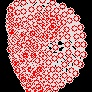
\includegraphics[width=\linewidth]{gambar/100 kanan.jpg}
      \caption{Citra kelas kanan}
      \label{fig:image1}
  \end{subfigure}
  \hfill
  \begin{subfigure}{0.3\textwidth}
      \centering
      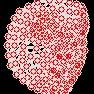
\includegraphics[width=\linewidth]{gambar/100 kiri.jpg}
      \caption{Citra kelas kiri}
      \label{fig:image2}
  \end{subfigure}
  \hfill
  \begin{subfigure}{0.3\textwidth}
      \centering
      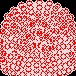
\includegraphics[width=\linewidth]{gambar/100 maju.jpg}
      \caption{Citra kelas maju}
      \label{fig:image3}
  \end{subfigure}
  
  \begin{subfigure}{0.3\textwidth}
      \centering
      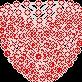
\includegraphics[width=\linewidth]{gambar/100 mundur.jpg}
      \caption{Citra kelas mundur}
      \label{fig:image4}
  \end{subfigure}
  \hfill
  \begin{subfigure}{0.3\textwidth}
      \centering
      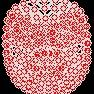
\includegraphics[width=\linewidth]{gambar/100 stop.jpg}
      \caption{Citra kelas \emph{stop}}
      \label{fig:image5}
  \end{subfigure}
  \caption{Dataset Jarak 100 sentimeter}
  \label{fig:15lux}
\end{figure}

Berdasarkan grafik yang didapat setelah dilakukan \emph{training}, model yag diambil dari jarak 100 sentimeter ini memiliki \emph{training accuracy} sebesar 80\% dan \emph{validation accuracy} sebesar 98.37\% seperti pada Gambar \ref{fig:AccuracyHasilPelatihanJarak100cm}. Model ini juga memiliki \emph{training loss} sebesar 0.3637 dan \emph{validation loss} sebesar 0.1045 yang dapat dilihat pada Gambar \ref{fig:LossHasilPelatihanJarak100cm}. Selain itu, dapat dilihat juga pada grafik bahwa \emph{training} yang dilakukan belum selesai di 15 \emph{epoch}. 


\begin{figure} [H] \centering
  % Nama dari file gambar yang diinputkan
  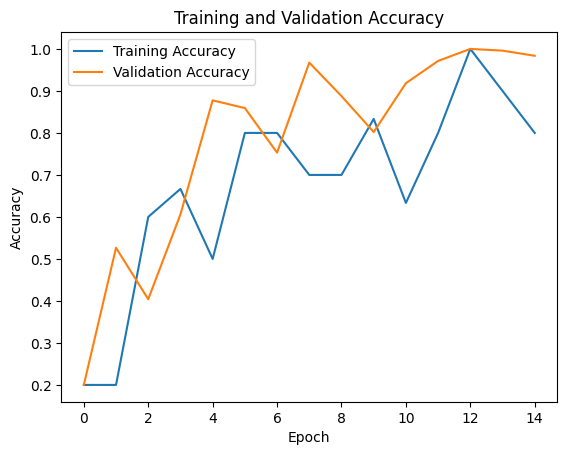
\includegraphics[scale=0.7]{gambar/100accuracy.png}
  % Keterangan gambar yang diinputkan
  \caption{Accuracy Hasil Pelatihan Jarak 100cm}
  % Label referensi dari gambar yang diinputkan
  \label{fig:AccuracyHasilPelatihanJarak100cm}
\end{figure}

\begin{figure} [H] \centering
  % Nama dari file gambar yang diinputkan
  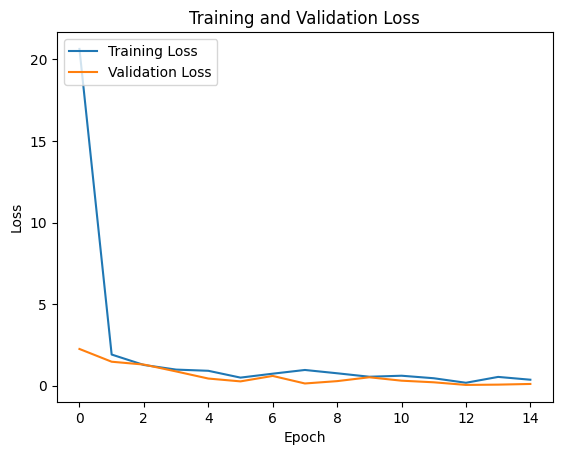
\includegraphics[scale=0.7]{gambar/100loss.png}
  % Keterangan gambar yang diinputkan
  \caption{Loss Hasil Pelatihan Jarak 100cm}
  % Label referensi dari gambar yang diinputkan
  \label{fig:LossHasilPelatihanJarak100cm}
\end{figure}


Dalam pengujian model CNN yang telah dibuat terhadap data validasi dan diambil dengan jarak 100 sentimeter, dengan menggunakan perhitungan \emph{confusion matrix}, didapatkan hasil klasifikasi seperti yang telah divisualisasikan pada Gambar \ref{fig:ConfusionMatrixHasilPelatihanJarak100cm}. Dari Gambar \ref{fig:ConfusionMatrixHasilPelatihanJarak100cm}, dapat dilihat bahwa dari 490 data pada model yang diujikan terhadap data citra validasi, terdapat 8 data citra yang hasil prediksinya tidak sesuai dengan data aktual yang diujikan. Delapan data citra tersebut merupakan data citra dari kelas kiri yang terdeteksi sebagai data citra dari kelas kanan. Persentase keberhasilan pada kelas kiri adalah sekitar 91,84\% dengan jumlah 90 data dan persentase ketidakberhasilannya adalah sekitar 8,16\% dengan jumlah 8 data. Pada Tabel \ref{tb:Hasil Validasi Nilai Model Jarak 100cm} dapat dilihat terdapat 8 data kelas kanan yang terdeteksi sebagai \emph{false positive} dan 384 data yang terdeteksi sebagai \emph{true negative}. Selain itu, dapat dilihat juga terdapat 8 data kelas kiri yang terdeteksi sebagai \emph{false negative} dan 90 data yang terdeteksi sebagai \emph{true positive}.

\begin{figure} [H] \centering
  % Nama dari file gambar yang diinputkan
  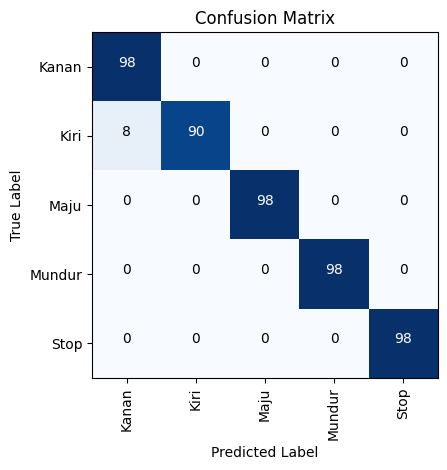
\includegraphics[scale=0.8]{gambar/100confusion.png}
  % Keterangan gambar yang diinputkan
  \caption{Confusion Matrix Hasil Pelatihan Jarak 100cm}
  % Label referensi dari gambar yang diinputkan
  \label{fig:ConfusionMatrixHasilPelatihanJarak100cm}
\end{figure}


    \begin{table}[H]
      \centering
      \caption{Hasil Klasifikasi Model Jarak 100cm}
      \label{tb:Hasil Klasifikasi Model Jarak 100cm}
    \begin{tabular}{|c|c|c|c|c|}
      \hline
      \rowcolor[HTML]{C0C0C0} 
      \cellcolor[HTML]{C0C0C0} & TP & TN  & FP & FN \\ \hline
      Kanan                    & 98 & 384 & 8  & 0  \\ \hline
      Kiri                     & 90 & 392 & 0  & 8  \\ \hline
      Maju                     & 98 & 392 & 0  & 0  \\ \hline
      Mundur                   & 98 & 392 & 0  & 0  \\ \hline
      Stop                     & 98 & 392 & 0  & 0  \\ \hline
      \end{tabular}
      \end{table}


Pada Tabel \ref{tb:Hasil Validasi Nilai Model Jarak 100cm} dapat dilihat bahwa nilai \emph{accuracy} pada kelas kanan adalah sebesar 0.9837 dan nilai \emph{precision}nya 0.9245. Hal ini menyebabkan kelas kanan memiliki \emph{F1-Score} sebesar 0.9608. Sedangkan pada kelas kiri, nilai \emph{accuracy}nya adalah 0.9837 dan nilai \emph{recall}nya 0.9184. Hal ini menyebabkan kelas kiri memiliki \emph{F1-Score} sebesar 0.9574. Pada kelas maju, mundur, dan \emph{stop} memiliki nilai \emph{accuracy}, \emph{precision}, \emph{recall}, dan \emph{F1-Score} sebesar 1.0000. 

\begin{table}[H]
  \centering
  \caption{Hasil Validasi Nilai Model Jarak 100cm}
  \label{tb:Hasil Validasi Nilai Model Jarak 100cm}
  \begin{tabular}{|c|c|c|c|c|}
    \hline
    \rowcolor[HTML]{C0C0C0} 
    \cellcolor[HTML]{C0C0C0} & Accuracy & Precision & Recall & F1-Score \\ \hline
    Kanan                    & 0.9837   & 0.9245    & 1.0000 & 0.9608   \\ \hline
    Kiri                     & 0.9837   & 1.0000    & 0.9184 & 0.9574   \\ \hline
    Maju                     & 1.0000   & 1.0000    & 1.0000 & 1.0000   \\ \hline
    Mundur                   & 1.0000   & 1.0000    & 1.0000 & 1.0000   \\ \hline
    Stop                     & 1.0000   & 1.0000    & 1.0000 & 1.0000   \\ \hline
    \end{tabular}
    \end{table}




\section{Pengujian performa model dengan variasi pencahayaan}
Pada bagian pengujian ini, penulis telah melakukan serangkaian uji coba untuk menggali pengaruh tingkat intensitas cahaya terhadap proses pendeteksian citra wajah secara real-time. Dalam hal ini, digunakan tiga level intensitas cahaya yang akan menjadi variabel bebas, yaitu 15 lux, 46 lux, dan 110 lux. Perbandingan keadaan ruangan secara \emph{real-time} dapat dilihat pada Tabel \ref{tab:VariasiIntensitasCahaya}.  Pengukuran nilai lux yang didapatkan dilakukan dengan menggunakan bantuan dari lightmeter yang terdapat di \emph{handphone} penulis untuk meningkatkan ketelitian pengukuran. Ketiga level intensitas Cahaya ini merepresentasikan tiga kondisi yang terdapat pada suatu ruangan. Dari dilakukannya pengujian dengan variasi intensitas cahaya ini diharapkan didapatkannya data mengenai adaptabilitas model pada kondisi pencahayaan yang berbeda-beda. Pada setiap pengujian akan dilakukan 460 kali pendeteksian yang mana kemudian akan dihitung perbandingan terdeteksi dan tidaknya pada intensitas cahaya yang sedang diujikan. Hasil yang didapatkan dari pengujian performa model dengan variasi pencahayaan yang telah dilakukan menunjukkan bahwa akurasi pendeteksian model yang paling tinggi adalah dalam keadaan ruangan dengan intensitas cahaya sebesar 110 lux yaitu keadaan pada saat malam hari dan semua lampu pada ruangan dinyalakan. Untuk pembahasan lebih detailnya mengenai penelitian ini dapat dilihat dari subbab masing-masing intensitas pencahayaan dibawah ini.

\begin{table}[H]
  \centering
  \begin{tabular}{|c|c|}
  \hline
  \textbf{Intensitas Cahaya} & \textbf{Keadaan Ruangan} \\ \hline
  15 & 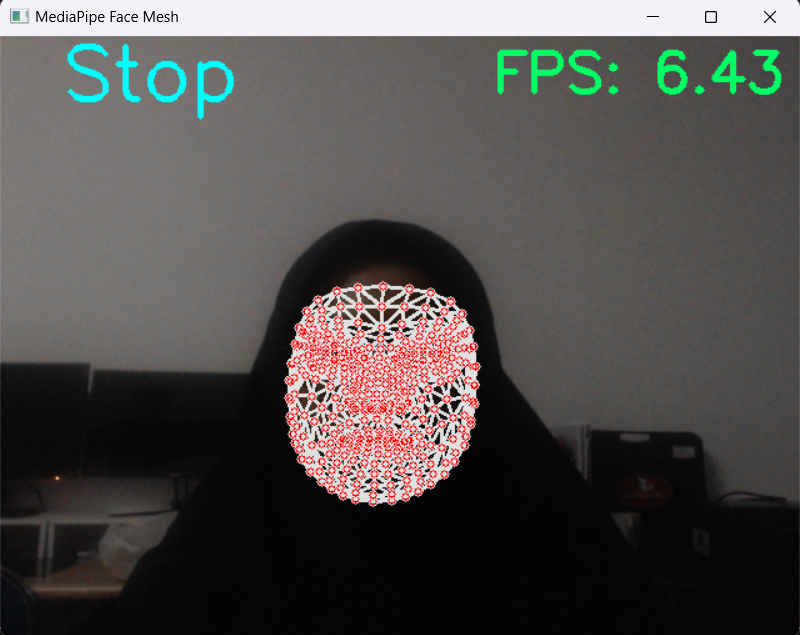
\includegraphics[width=0.3\textwidth]{gambar/15 stop.png} \\ \hline
  46 & 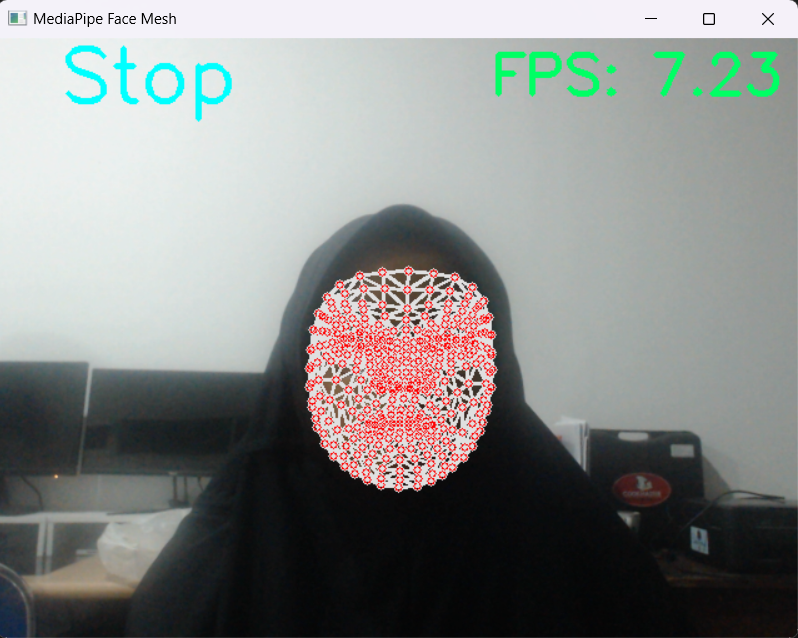
\includegraphics[width=0.3\textwidth]{gambar/46 stop.png} \\ \hline
  110 & 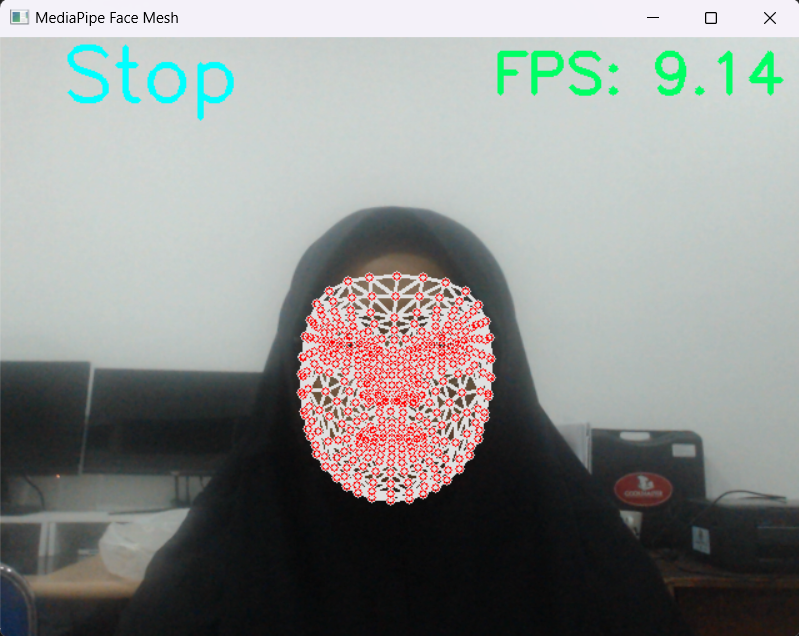
\includegraphics[width=0.3\textwidth]{gambar/110 stop.png} \\ \hline
  \end{tabular}
  \caption{Variasi Intensitas Cahaya}
  \label{tab:VariasiIntensitasCahaya}
  \end{table}

\subsection{Pengujian intensitas cahaya 15 lux}
Pengujian pertama dilakukan dengan menguji intensitas cahaya sebesar 15 lux yang merepresentasikan kondisi dalam ruangan dengan lampu mati pada malam hari kemudian dinyalakan sebuah senter yang dihadapkan kearah langit-langit ruangan. Gambar \ref{fig:15lux} menunjukkan keadaan pada saat cahaya dengan intensitas 15 lux ketika dilakukannya pengujian ini.

\begin{figure}[H]
  \centering
  \begin{subfigure}{0.3\textwidth}
      \centering
      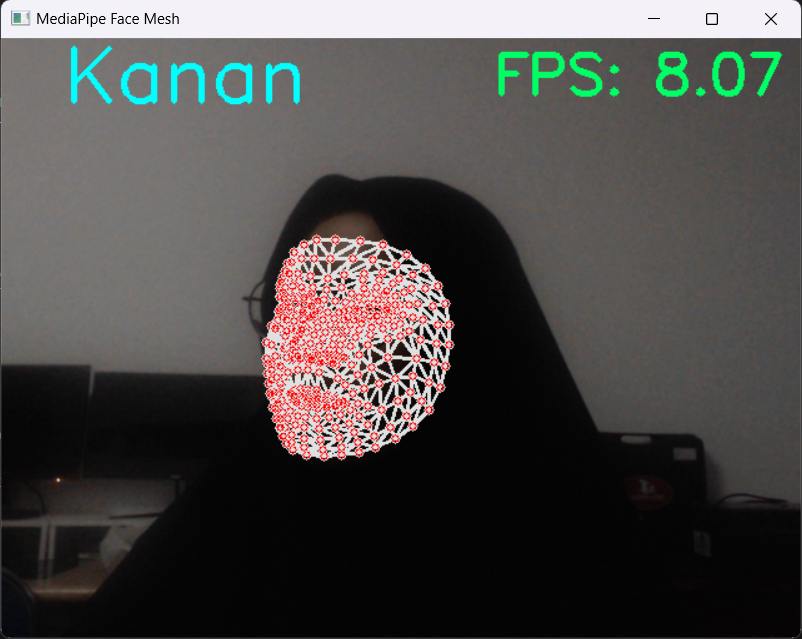
\includegraphics[width=\linewidth]{gambar/15 kanan.png}
      \caption{Citra kelas kanan}
      \label{fig:image1}
  \end{subfigure}
  \hfill
  \begin{subfigure}{0.3\textwidth}
      \centering
      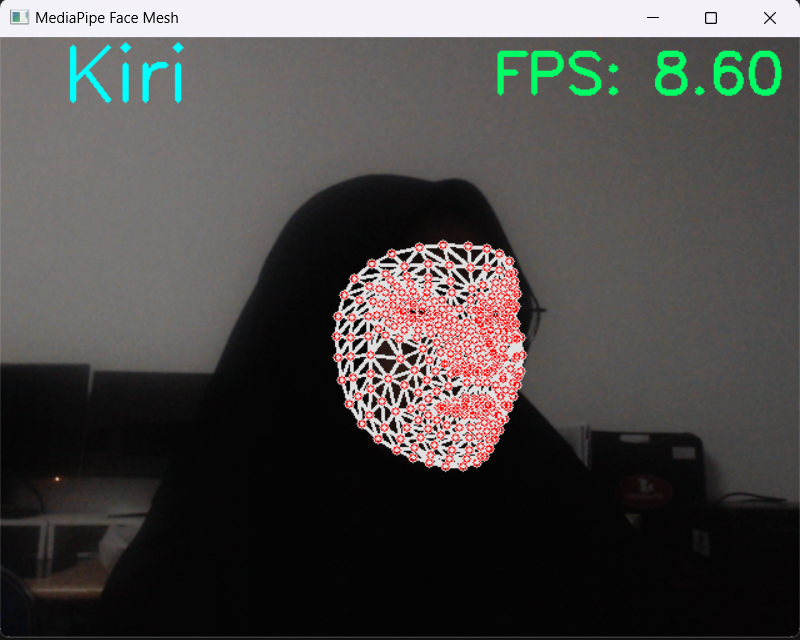
\includegraphics[width=\linewidth]{gambar/15 kiri.png}
      \caption{Citra kelas kiri}
      \label{fig:image2}
  \end{subfigure}
  \hfill
  \begin{subfigure}{0.3\textwidth}
      \centering
      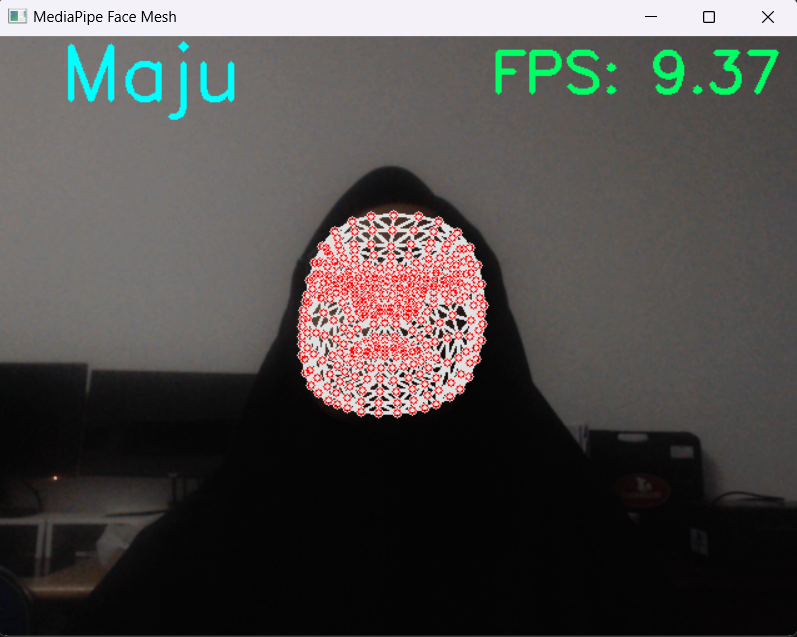
\includegraphics[width=\linewidth]{gambar/15 maju.png}
      \caption{Citra kelas maju}
      \label{fig:image3}
  \end{subfigure}
  
  \begin{subfigure}{0.3\textwidth}
      \centering
      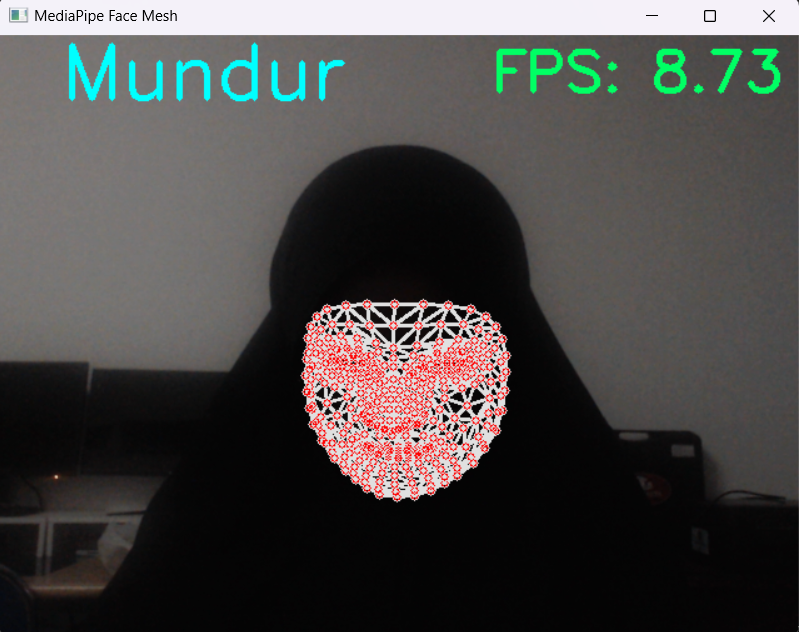
\includegraphics[width=\linewidth]{gambar/15 mundur.png}
      \caption{Citra kelas mundur}
      \label{fig:image4}
  \end{subfigure}
  \hfill
  \begin{subfigure}{0.3\textwidth}
      \centering
      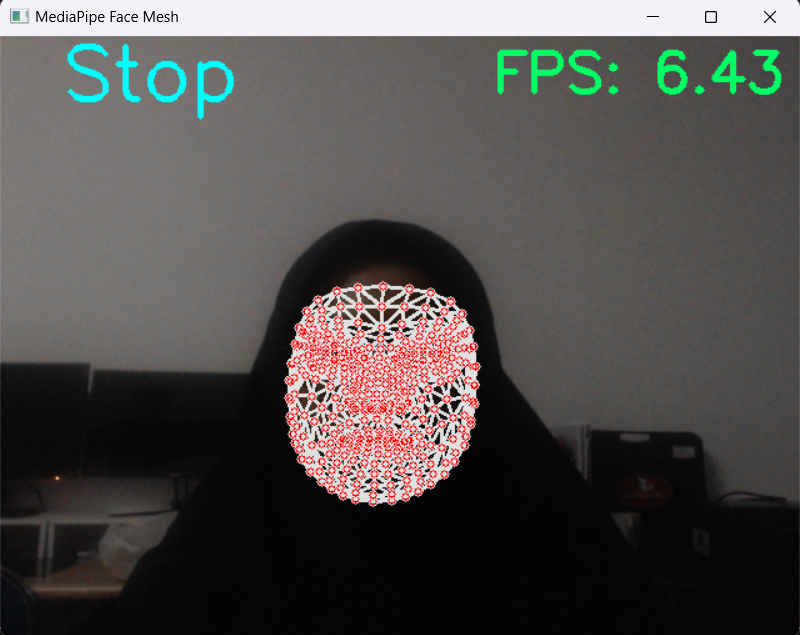
\includegraphics[width=\linewidth]{gambar/15 stop.png}
      \caption{Citra kelas \emph{stop}}
      \label{fig:image5}
  \end{subfigure}
  \caption{Pendeteksian pada 15 lux}
  \label{fig:15lux}
\end{figure}

Hasil yang didapatkan dari proses pengujian ini menunjukkan tingkat akurasi yang cukup baik, yaitu sekitar 95,87\% dari 460 kali pendeteksian yang dilakukan. Hal ini menunjukkan bahwa dari 460 kali pendeteksian yang dilakukan, 441 kali diantaranya berhasil terdeteksi dan 19 lainnya tidak berhasil terdeteksi. Informasi mengenai performa ini telah di representasikan pada Tabel \ref{tb:15lux}. Hasil yang diperoleh dari pengujian ini menunjukkan bahwa meskipun kondisi cahaya dan penerangannya sangat minim di sekitar 15 lux, kamera masih dapat mendeteksi citra wajah dan model masih mampu memproses landmark-landmark pada citra wajah dan kemudian melakukan klasifikasi untuk pose wajah yang sedang dideteksi dengan akurasi yang cukup baik. Hal ini memperlihatkan kemampuan model untuk beradaptasi terhadap intensitas pencahayaan suatu ruangan sehingga model tidak bergantung pada tingkat pencahayaan tertentu.

\begin{longtable}{|c|c|}
  \caption{Hasil Variasi 15 Lux}
  \label{tb:15lux}   \\
  \hline
  \cellcolor[HTML]{C0C0C0}
  \textbf{Jumlah Keberhasilan:} & 441\\
  \hline
  \cellcolor[HTML]{C0C0C0}
  \textbf{Jumlah Ketidakberhasilan:} & 19\\
  \hline
  \cellcolor[HTML]{C0C0C0}
  \textbf{Persentasi Keberhasilan:} & 95,87\% \\
  \hline
  \cellcolor[HTML]{C0C0C0}
  \textbf{Persentasi Ketidakberhasilan:} & 4,13\% \\
  \hline
  \end{longtable}


\subsection{Pengujian intensitas cahaya 46 lux}
Pengujian kedua dilakukan dengan menguji tingkat intensitas cahaya sebesar 46 lux yang merepresentasikan kondisi dalam ruangan pada malam hari yang setengah lampunya dinyalakan dan setengah lainnya dimatikan. Gambar \ref{fig:46lux} menunjukkan keadaan pada saat cahaya dengan intensitas 46 lux ketika dilakukannya pengujian ini.


\begin{figure}[H]
  \centering
  \begin{subfigure}{0.3\textwidth}
      \centering
      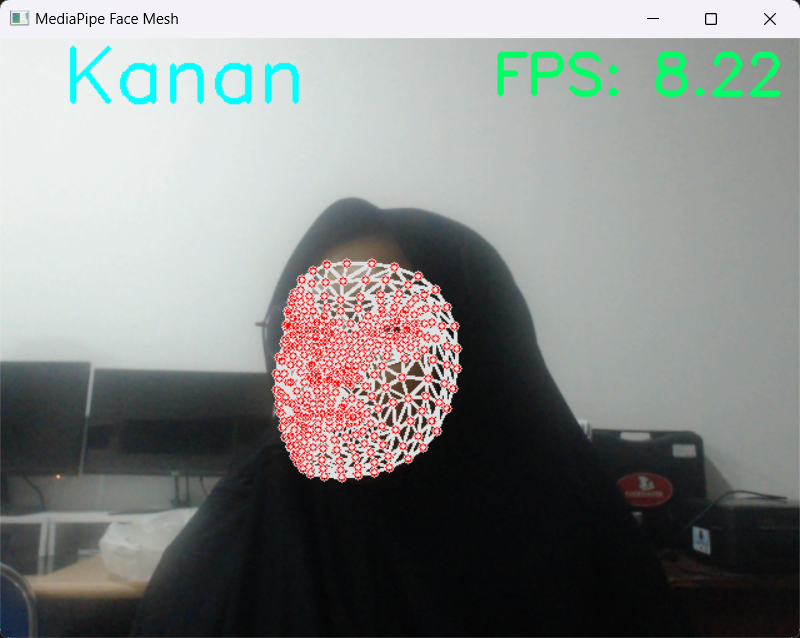
\includegraphics[width=\linewidth]{gambar/46 kanan.png}
      \caption{Citra kelas kanan}
      \label{fig:image1}
  \end{subfigure}
  \hfill
  \begin{subfigure}{0.3\textwidth}
      \centering
      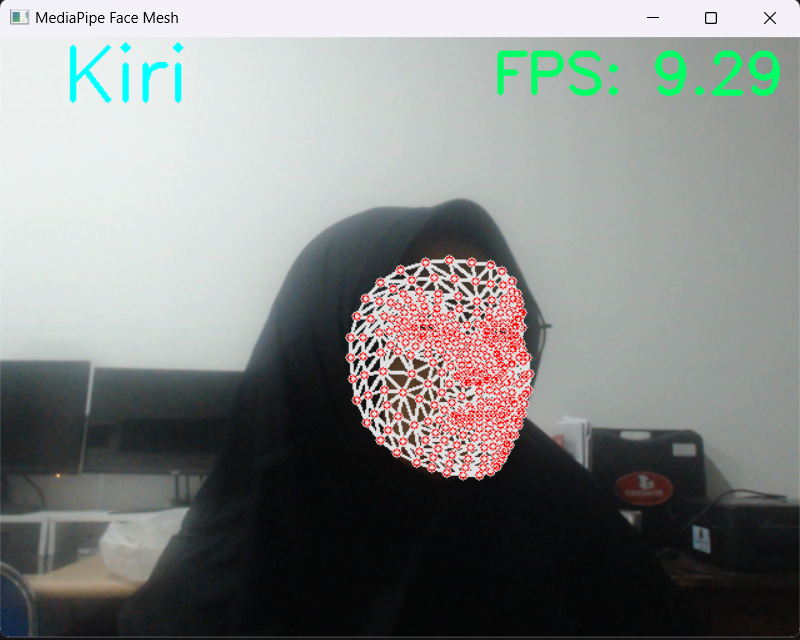
\includegraphics[width=\linewidth]{gambar/46 kiri.png}
      \caption{Citra kelas kiri}
      \label{fig:image2}
  \end{subfigure}
  \hfill
  \begin{subfigure}{0.3\textwidth}
      \centering
      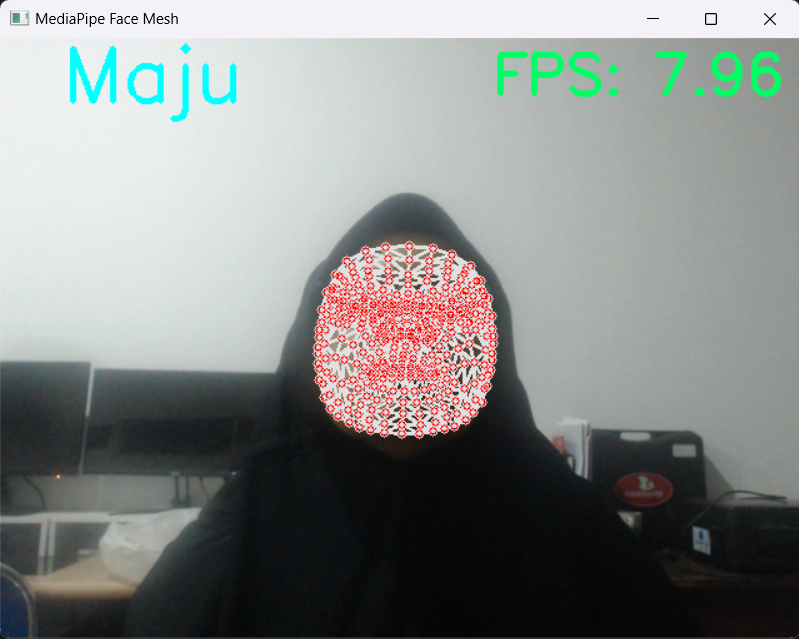
\includegraphics[width=\linewidth]{gambar/46 maju.png}
      \caption{Citra kelas maju}
      \label{fig:image3}
  \end{subfigure}
  
  \begin{subfigure}{0.3\textwidth}
      \centering
      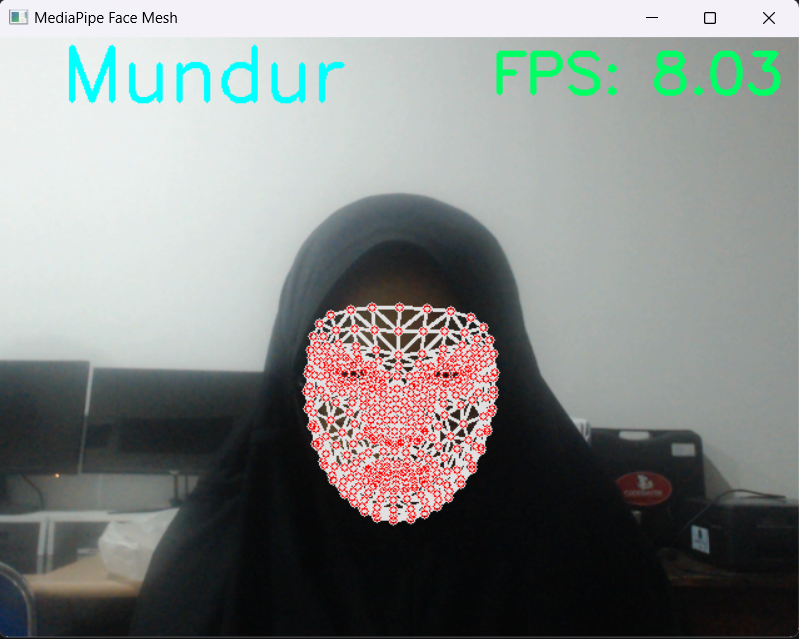
\includegraphics[width=\linewidth]{gambar/46 mundur.png}
      \caption{Citra kelas mundur}
      \label{fig:image4}
  \end{subfigure}
  \hfill
  \begin{subfigure}{0.3\textwidth}
      \centering
      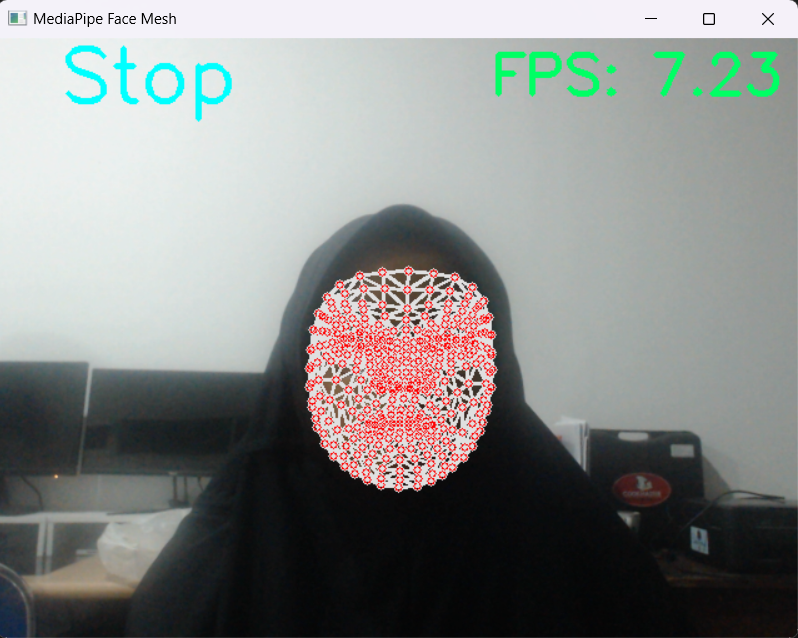
\includegraphics[width=\linewidth]{gambar/46 stop.png}
      \caption{Citra kelas \emph{stop}}
      \label{fig:image5}
  \end{subfigure}
  \caption{Pendeteksian pada 46 lux}
  \label{fig:46lux}
\end{figure}

Hasil yang didapatkan dari proses pengujian ini menunjukkan tingkat akurasi yang sangat baik, yaitu sekitar 95,87\% dari 460 kali pendeteksian yang dilakukan. Hal ini menunjukkan bahwa dari 460 kali pendeteksian yang dilakukan, 458 kali diantaranya berhasil terdeteksi dan 2 lainnya tidak berhasil terdeteksi. Informasi mengenai performa ini telah di representasikan pada Tabel \ref{tb:46lux}. Hasil yang diperoleh dari pengujian ini menunjukkan bahwa ketika kondisi cahaya dan penerangannya remang-remang atau sekitar 46 lux, kamera dapat mendeteksi citra wajah dan model mampu memproses landmark-landmark pada citra wajah dan kemudian melakukan klasifikasi untuk pose wajah yang sedang dideteksi dengan akurasi yang sangat baik. Hal ini memperlihatkan kemampuan model untuk beradaptasi terhadap intensitas pencahayaan suatu ruangan sehingga model tidak terikat pada tingkat pencahayaan tertentu.

\begin{longtable}{|c|c|}
  \caption{Hasil Variasi 46 Lux}
  \label{tb:46lux}\\
  \hline
  \cellcolor[HTML]{C0C0C0}
  \textbf{Jumlah Keberhasilan:} & 458\\
  \hline
  \cellcolor[HTML]{C0C0C0}
  \textbf{Jumlah Ketidakberhasilan:} & 2\\
  \hline
  \cellcolor[HTML]{C0C0C0}
  \textbf{Persentasi Keberhasilan:} & 99,57\% \\
  \hline
  \cellcolor[HTML]{C0C0C0}
  \textbf{Persentasi Ketidakberhasilan:} & 0,43\% \\
  \hline
  \end{longtable}

\subsection{Pengujian intensitas cahaya 110 lux}
Pengujian ketiga dilakukan dengan menguji tingkat intensitas cahaya sebesar 110 lux, merepresentasikan kondisi dalam ruangan pada malam hari yang semua lampunya dinyalakan. Gambar \ref{fig:110lux} menunjukkan keadaan pada saat cahaya dengan intensitas 46 lux ketika dilakukannya pengujian ini.


\begin{figure}[H]
  \centering
  \begin{subfigure}{0.3\textwidth}
      \centering
      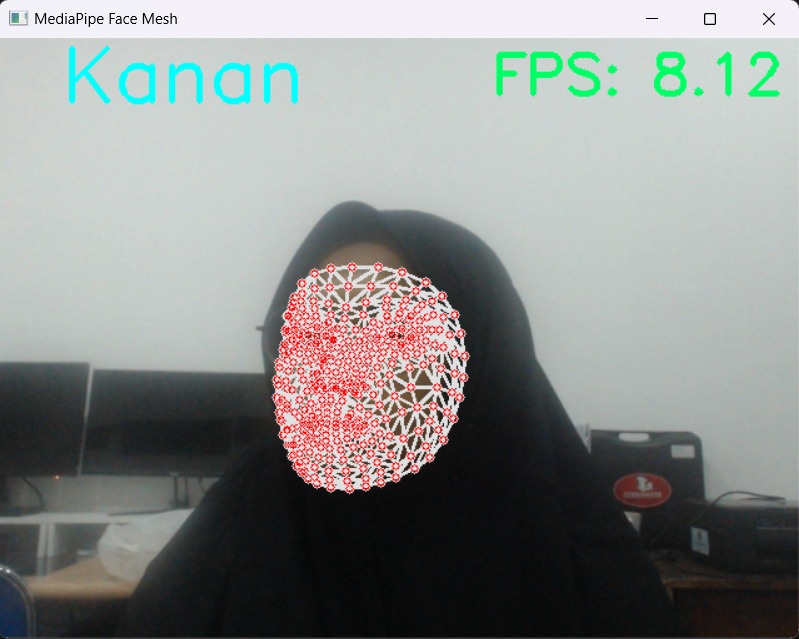
\includegraphics[width=\linewidth]{gambar/110 kanan.png}
      \caption{Citra kelas kanan}
      \label{fig:image1}
  \end{subfigure}
  \hfill
  \begin{subfigure}{0.3\textwidth}
      \centering
      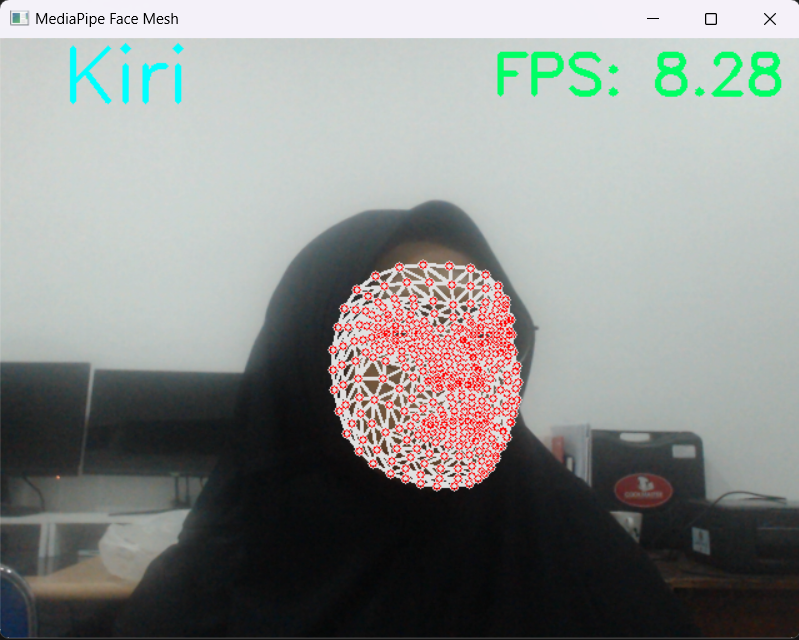
\includegraphics[width=\linewidth]{gambar/110 kiri.png}
      \caption{Citra kelas kiri}
      \label{fig:image2}
  \end{subfigure}
  \hfill
  \begin{subfigure}{0.3\textwidth}
      \centering
      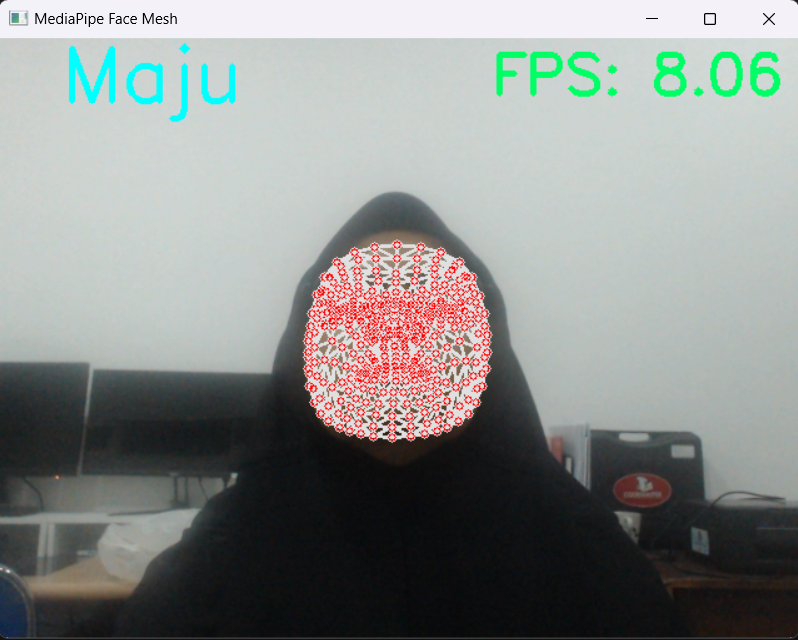
\includegraphics[width=\linewidth]{gambar/110 maju.png}
      \caption{Citra kelas maju}
      \label{fig:image3}
  \end{subfigure}
  
  \begin{subfigure}{0.3\textwidth}
      \centering
      \includegraphics[width=\linewidth]{gambar/110 mundur.png}
      \caption{Citra kelas mundur}
      \label{fig:image4}
  \end{subfigure}
  \hfill
  \begin{subfigure}{0.3\textwidth}
      \centering
      \includegraphics[width=\linewidth]{gambar/110 stop.png}
      \caption{Citra kelas \emph{stop}}
      \label{fig:image5}
  \end{subfigure}
  \caption{Pendeteksian pada 110 lux}
  \label{fig:110lux}
\end{figure}

Hasil yang didapatkan dari proses pengujian ini menunjukkan tingkat akurasi yang sangat baik, yaitu sekitar 99,78\% dari 460 kali pendeteksian yang dilakukan. Hal ini menunjukkan bahwa dari 460 kali pendeteksian yang dilakukan, 459 kali diantaranya berhasil terdeteksi dan 1 lainnya tidak berhasil terdeteksi. Informasi mengenai performa ini telah di representasikan pada Tabel \ref{tb:100lux}. Hasil yang diperoleh dari pengujian ini menunjukkan bahwa ketika kondisi cahaya dan penerangannya terang atau sekitar 110 lux, kamera dapat dengan mudah mendeteksi citra wajah sehingga model mampu memproses landmark-landmark pada citra wajah dengan sangat baik. Proses klasifikasi untuk pose wajah yang sedang dideteksi juga memiliki tingkat akurasi yang sangat tinggi. Hal ini menunjukkan bahwa model dapat bekerja dengan sangat baik pada ruangan yang terang.

\begin{longtable}{|c|c|}
  \caption{Hasil Variasi 110 Lux}
  \label{tb:110lux}   \\
  \hline
  \cellcolor[HTML]{C0C0C0}
  \textbf{Jumlah Keberhasilan:} & 459\\
  \hline
  \cellcolor[HTML]{C0C0C0}
  \textbf{Jumlah Ketidakberhasilan:} & 1\\
  \hline
  \cellcolor[HTML]{C0C0C0}
  \textbf{Persentasi Keberhasilan:} & 99,78\% \\
  \hline
  \cellcolor[HTML]{C0C0C0}
  \textbf{Persentasi Ketidakberhasilan:} & 0,22\% \\
  \hline
  \end{longtable}

\section{Pengujian Kecepatan FPS}
Dalam skenario pengujian ini, akan dilakukan dua kali pengujian. Pengujian pertama akan dilakukan pada laptop penulis dan pengujian kedua akan dilakukan pada NUC yang mana hal ini menjadikan laptop dan NUC menjadi variabel bebas dari skenario pengujian kali ini. Pada pengujian ini kecepatan FPS yang akan dijadikan variabel terikatnya. Skenario pengujian ini akan dilakukan selama 1 menit untuk setiap pengujiannya.


\subsection{Pengujian Kecepatan FPS Pada Laptop}
Pada pengujian ini, dilakukan pengambilan data FPS selama 60 detik dengan menggunakan laptop penulis. Didapatkan nilai rata-rata FPS pada laptop sebesar 7.645666667. Pengambilan data pengujian dilakukan dengan menggunakan perangkat dengan spesifikasi yang telah dijabarkan pada Tabel \ref{tb:SpesifikasiLaptop}.

Selama dilakukannya pengujian pada FPS laptop, didapatkan FPS paling tinggi sebesar 12.13 dan FPS paling rendahnya sebesar 3.25. Data lengkap yang didapatkan dari pengujian ini dapat dilihat pada Tabel \ref{tb:HasilPengujianFPSLaptop}.


\begin{longtable}{|c|c|}
  \caption{Spesifikasi Laptop}
  \label{tb:SpesifikasiLaptop}                                   \\
  \hline
  \rowcolor[HTML]{C0C0C0}
  \textbf{Komponen} & \textbf{Tipe} \\
  \hline
  CPU         & Intel(R) Core(TM) Ultra 7 155H              \\
  \hline
  RAM         & 16 GB DDR5-5600              \\
  \hline
  OS         & Windows 11 Home Single Language              \\
  \hline
\end{longtable}


\begin{table}[H]
  \centering
  \caption{Hasil Pengujian FPS Laptop}
  \label{tb:HasilPengujianFPSLaptop}
  \begin{tabular}{|r|r|l|r|r|}
  \cline{1-2} \cline{4-5}
  \multicolumn{1}{|l|}{\cellcolor[HTML]{C0C0C0}\textbf{No}} & \multicolumn{1}{l|}{\cellcolor[HTML]{C0C0C0}\textbf{FPS}} &  & \multicolumn{1}{l|}{\cellcolor[HTML]{C0C0C0}{\color[HTML]{000000} \textbf{No}}} & \multicolumn{1}{l|}{\cellcolor[HTML]{C0C0C0}{\color[HTML]{000000} \textbf{FPS}}} \\ \cline{1-2} \cline{4-5} 
  1                                                         & 9.38                                                      &  & 31                                                                              & 7.23                                                                             \\ \cline{1-2} \cline{4-5} 
  2                                                         & 7.18                                                      &  & 32                                                                              & 3.53                                                                             \\ \cline{1-2} \cline{4-5} 
  3                                                         & 6.13                                                      &  & 33                                                                              & 8.1                                                                              \\ \cline{1-2} \cline{4-5} 
  4                                                         & 8.72                                                      &  & 34                                                                              & 8.1                                                                              \\ \cline{1-2} \cline{4-5} 
  5                                                         & 9.4                                                       &  & 35                                                                              & 5.84                                                                             \\ \cline{1-2} \cline{4-5} 
  6                                                         & 9.36                                                      &  & 36                                                                              & 5.6                                                                              \\ \cline{1-2} \cline{4-5} 
  7                                                         & 7.64                                                      &  & 37                                                                              & 7.23                                                                             \\ \cline{1-2} \cline{4-5} 
  8                                                         & 6.81                                                      &  & 38                                                                              & 9.4                                                                              \\ \cline{1-2} \cline{4-5} 
  9                                                         & 7.07                                                      &  & 39                                                                              & 7.26                                                                             \\ \cline{1-2} \cline{4-5} 
  10                                                        & 9.4                                                       &  & 40                                                                              & 9.37                                                                             \\ \cline{1-2} \cline{4-5} 
  11                                                        & 8.66                                                      &  & 41                                                                              & 5.61                                                                             \\ \cline{1-2} \cline{4-5} 
  12                                                        & 3.25                                                      &  & 42                                                                              & 8.18                                                                             \\ \cline{1-2} \cline{4-5} 
  13                                                        & 8.13                                                      &  & 43                                                                              & 5.56                                                                             \\ \cline{1-2} \cline{4-5} 
  14                                                        & 9.4                                                       &  & 44                                                                              & 9.4                                                                              \\ \cline{1-2} \cline{4-5} 
  15                                                        & 10.69                                                     &  & 45                                                                              & 6.41                                                                             \\ \cline{1-2} \cline{4-5} 
  16                                                        & 6.82                                                      &  & 46                                                                              & 5.77                                                                             \\ \cline{1-2} \cline{4-5} 
  17                                                        & 8.55                                                      &  & 47                                                                              & 6.15                                                                             \\ \cline{1-2} \cline{4-5} 
  18                                                        & 7.97                                                      &  & 48                                                                              & 4.94                                                                             \\ \cline{1-2} \cline{4-5} 
  19                                                        & 9.92                                                      &  & 49                                                                              & 7.62                                                                             \\ \cline{1-2} \cline{4-5} 
  20                                                        & 9.34                                                      &  & 50                                                                              & 8.08                                                                             \\ \cline{1-2} \cline{4-5} 
  21                                                        & 8.14                                                      &  & 51                                                                              & 9.26                                                                             \\ \cline{1-2} \cline{4-5} 
  22                                                        & 6.8                                                       &  & 52                                                                              & 6.67                                                                             \\ \cline{1-2} \cline{4-5} 
  23                                                        & 7.91                                                      &  & 53                                                                              & 10.03                                                                            \\ \cline{1-2} \cline{4-5} 
  24                                                        & 3.95                                                      &  & 54                                                                              & 8.72                                                                             \\ \cline{1-2} \cline{4-5} 
  25                                                        & 4.74                                                      &  & 55                                                                              & 7.55                                                                             \\ \cline{1-2} \cline{4-5} 
  26                                                        & 8.53                                                      &  & 56                                                                              & 8.72                                                                             \\ \cline{1-2} \cline{4-5} 
  27                                                        & 6.39                                                      &  & 57                                                                              & 5.89                                                                             \\ \cline{1-2} \cline{4-5} 
  28                                                        & 8.74                                                      &  & 58                                                                              & 9.4                                                                              \\ \cline{1-2} \cline{4-5} 
  29                                                        & 8.17                                                      &  & 59                                                                              & 7.67                                                                             \\ \cline{1-2} \cline{4-5} 
  30                                                        & 12.13                                                     &  & 60                                                                              & 6.13                                                                             \\ \cline{1-2} \cline{4-5} 
  \end{tabular}
  \end{table}

\subsection{Pengujian Kecepatan FPS Pada NUC}
Pada pengujian ini, dilakukan pengambilan data FPS selama 60 detik dengan menggunakan NUC. Didapatkan nilai rata-rata FPS pada NUC sebesar 6.314. Pengambilan data pengujian dilakukan dengan menggunakan perangkat dengan spesifikasi yang telah dijabarkan pada Tabel \ref{tb:SpesifikasiNUC}. Hal ini menunjukkan bahwa laptop penulis memiliki kekuatan pemrosesan yang lebih baik daripada NUC yang digunakan pada penelitian kali ini. Meskipun perbedaan rata-rata FPS antara laptop penulis dan NUC yang digunakan tidak jauh, hanya sekitar 1.331667.

Selama dilakukannya pengujian pada FPS NUC, didapatkan FPS paling tinggi sebesar 7.79 dan FPS paling rendahnya sebesar 2.24. Data lengkap yang didapatkan dari pengujian ini dapat dilihat pada Tabel \ref{tb:HasilPengujianFPSNUC}.

\begin{longtable}{|c|c|}
  \caption{Spesifikasi NUC}
  \label{tb:SpesifikasiNUC}                                   \\
  \hline
  \rowcolor[HTML]{C0C0C0}
  \textbf{Komponen} & \textbf{Tipe} \\
  \hline
  CPU         & Intel® Core™ i7-1165G7              \\
  \hline
  RAM         & 32 GB LPDDR4              \\
  \hline
  OS         & Windows 11 Home Single Language              \\
  \hline
\end{longtable}



\begin{table}[H]
\centering
  \caption{Hasil Pengujian FPS NUC}
  \label{tb:HasilPengujianFPSNUC}
  \begin{tabular}{|r|r|l|r|r|}
  \cline{1-2} \cline{4-5}
  \multicolumn{1}{|l|}{\cellcolor[HTML]{C0C0C0}\textbf{No}} & \multicolumn{1}{l|}{\cellcolor[HTML]{C0C0C0}\textbf{FPS}} &  & \multicolumn{1}{l|}{\cellcolor[HTML]{C0C0C0}{\color[HTML]{000000} \textbf{No}}} & \multicolumn{1}{l|}{\cellcolor[HTML]{C0C0C0}{\color[HTML]{000000} \textbf{FPS}}} \\ \cline{1-2} \cline{4-5} 
  1                                                         & 6.67                                                      &  & 31                                                                              & 5.9                                                                              \\ \cline{1-2} \cline{4-5} 
  2                                                         & 5.56                                                      &  & 32                                                                              & 5.18                                                                             \\ \cline{1-2} \cline{4-5} 
  3                                                         & 4.99                                                      &  & 33                                                                              & 6.07                                                                             \\ \cline{1-2} \cline{4-5} 
  4                                                         & 7.79                                                      &  & 34                                                                              & 5.93                                                                             \\ \cline{1-2} \cline{4-5} 
  5                                                         & 6.06                                                      &  & 35                                                                              & 7.31                                                                             \\ \cline{1-2} \cline{4-5} 
  6                                                         & 5.41                                                      &  & 36                                                                              & 7.41                                                                             \\ \cline{1-2} \cline{4-5} 
  7                                                         & 6.49                                                      &  & 37                                                                              & 6.53                                                                             \\ \cline{1-2} \cline{4-5} 
  8                                                         & 6.6                                                       &  & 38                                                                              & 7.28                                                                             \\ \cline{1-2} \cline{4-5} 
  9                                                         & 6.42                                                      &  & 39                                                                              & 2.24                                                                             \\ \cline{1-2} \cline{4-5} 
  10                                                        & 7.23                                                      &  & 40                                                                              & 6.96                                                                             \\ \cline{1-2} \cline{4-5} 
  11                                                        & 5.45                                                      &  & 41                                                                              & 6.65                                                                             \\ \cline{1-2} \cline{4-5} 
  12                                                        & 6.75                                                      &  & 42                                                                              & 7.29                                                                             \\ \cline{1-2} \cline{4-5} 
  13                                                        & 6.6                                                       &  & 43                                                                              & 6.57                                                                             \\ \cline{1-2} \cline{4-5} 
  14                                                        & 6.6                                                       &  & 44                                                                              & 7.32                                                                             \\ \cline{1-2} \cline{4-5} 
  15                                                        & 5.64                                                      &  & 45                                                                              & 6.92                                                                             \\ \cline{1-2} \cline{4-5} 
  16                                                        & 5.84                                                      &  & 46                                                                              & 4.93                                                                             \\ \cline{1-2} \cline{4-5} 
  17                                                        & 5.26                                                      &  & 47                                                                              & 7.57                                                                             \\ \cline{1-2} \cline{4-5} 
  18                                                        & 6.59                                                      &  & 48                                                                              & 6.46                                                                             \\ \cline{1-2} \cline{4-5} 
  19                                                        & 5.88                                                      &  & 49                                                                              & 5.55                                                                             \\ \cline{1-2} \cline{4-5} 
  20                                                        & 7.05                                                      &  & 50                                                                              & 7.65                                                                             \\ \cline{1-2} \cline{4-5} 
  21                                                        & 7.35                                                      &  & 51                                                                              & 5.53                                                                             \\ \cline{1-2} \cline{4-5} 
  22                                                        & 6.91                                                      &  & 52                                                                              & 6.57                                                                             \\ \cline{1-2} \cline{4-5} 
  23                                                        & 7.43                                                      &  & 53                                                                              & 2.76                                                                             \\ \cline{1-2} \cline{4-5} 
  24                                                        & 3.31                                                      &  & 54                                                                              & 6.68                                                                             \\ \cline{1-2} \cline{4-5} 
  25                                                        & 7.81                                                      &  & 55                                                                              & 6.86                                                                             \\ \cline{1-2} \cline{4-5} 
  26                                                        & 6.66                                                      &  & 56                                                                              & 6.72                                                                             \\ \cline{1-2} \cline{4-5} 
  27                                                        & 5.35                                                      &  & 57                                                                              & 7.27                                                                             \\ \cline{1-2} \cline{4-5} 
  28                                                        & 6.77                                                      &  & 58                                                                              & 4.73                                                                             \\ \cline{1-2} \cline{4-5} 
  29                                                        & 7.21                                                      &  & 59                                                                              & 6.78                                                                             \\ \cline{1-2} \cline{4-5} 
  30                                                        & 6.83                                                      &  & 60                                                                              & 6.71                                                                             \\ \cline{1-2} \cline{4-5} 
  \end{tabular}
\end{table}

\section{Pengujian Waktu Respons Kontrol Kursi Roda}
Pada pengujian ini, dilakukan perhitungan lama waktu yang dibutuhkan untuk melakukan pendeteksian dengan model yang kemudian diklasifikasikan dan dikirim ke ESP32 hingga motor kursi roda mulai bergerak. Pengujian ini dilakukan secara real-time. Perhitungan waktu \emph{delay} adalah dari timestamp mulai dikirimnya data hingga timestamp berhentinya motor kursi roda, sedangkan perhitungan \emph{inference time} dimulai dari dimulainya proses prediksi hingga didapatkan hasil dari proses klasifikasi. Rata-rata waktu \emph{delay} yang didapatkan adalah 0,3025423729. Dari data hasil yang telah didapatkan dan dijabarkan pada Tabel \ref{tb:HasilPengujianResponsTime}, dapat dilihat bahwa waktu delay terlama adalah 0,784 dan waktu delay tersingkatnya adalah 0,008. Nilai \emph{inference time} rata-rata yang didapatkan dari pengujian kali ini adalah sekitar 0,07220. Dapat dilihat juga dari Tabel \ref{tb:HasilPengujianResponsTime} bahwa waktu terlama yang diperlukan untuk melakukan inferensi adalah 0.17112 dan waktu tersingkat yang diperlukan adalah 0.6040. 

Dari Tabel \ref{tb:HasilPengujianResponsTime} didapatkan juga rata-rata delay untuk tiap-tiap kelasnya. Rata-rata waktu delay yang didapatkan untuk kelas kanan adalah 0,1664285714 detik dari 7 kelas kanan yang diujikan. Rata-rata waktu delay yang didapatkan untuk kelas kiri adalah 0,2398888889 detik dari 9 kelas kiri yang diujikan. Rata-rata waktu delay yang didapatkan untuk kelas maju adalah 0,4099 detik dari 10 kelas maju yang diujikan. Rata-rata waktu delay yang didapatkan untuk kelas mundur adalah 0,195 detik dari 3 kelas mundur yang diujikan. Rata-rata waktu delay yang didapatkan untuk kelas \emph{stop} adalah 0,3280666667 detik dari 30 kelas \emph{stop} yang diujikan. Terdapat 30 data kelas \emph{stop} dari 60 data yang ada karena setiap kali akan mengganti arah harus melakukan arah \emph{stop} terlebih dahulu.

Selain itu, dari Tabel \ref{tb:HasilPengujianResponsTime} didapatkan juga rata-rata \emph{inference time} untuk tiap-tiap kelasnya. Rata-rata waktu \emph{inference time} yang didapatkan untuk kelas kanan adalah 0,07392142857 detik dari 7 kelas kanan yang diujikan. Rata-rata waktu \emph{inference time} yang didapatkan untuk kelas kiri adalah 0,07187444444 detik dari 9 kelas kiri yang diujikan. Rata-rata waktu \emph{inference time} yang didapatkan untuk kelas maju adalah 0,080469 detik dari 10 kelas maju yang diujikan. Rata-rata waktu \emph{inference time} yang didapatkan untuk kelas mundur adalah 0,07338333333 detik dari 3 kelas mundur yang diujikan. Rata-rata waktu \emph{inference time} yang didapatkan untuk kelas \emph{stop} adalah 0,069029 detik dari 30 kelas \emph{stop} yang diujikan.


\begin{longtable}{|l|l|l|l|l|l|}
  \caption{Hasil Pengujian Respons Time}\label{tb:HasilPengujianResponsTime} \\
  \hline
  \rowcolor[HTML]{C0C0C0} 
  \multicolumn{1}{|c|}{\cellcolor[HTML]{C0C0C0}\begin{tabular}[c]{@{}c@{}}Inference \\ Time\end{tabular}} & \multicolumn{1}{c|}{\cellcolor[HTML]{C0C0C0}\begin{tabular}[c]{@{}c@{}}Timestamp \\ Sent\end{tabular}} & \multicolumn{1}{c|}{\cellcolor[HTML]{C0C0C0}\begin{tabular}[c]{@{}c@{}}Timestamp \\ Received\end{tabular}} & \multicolumn{1}{c|}{\cellcolor[HTML]{C0C0C0}\begin{tabular}[c]{@{}c@{}}Timestamp \\ Motor\end{tabular}} & \multicolumn{1}{c|}{\cellcolor[HTML]{C0C0C0}Delay} & \multicolumn{1}{c|}{\cellcolor[HTML]{C0C0C0}Arah} \\ 
  \endfirsthead
  
  \multicolumn{6}{c}%
  {{\bfseries Table \thetable\ dilanjutkan dari halaman sebelumnya}} \\
  \hline
  \rowcolor[HTML]{C0C0C0} 
  \multicolumn{1}{|c|}{\cellcolor[HTML]{C0C0C0}\begin{tabular}[c]{@{}c@{}}Inference \\ Time\end{tabular}} & \multicolumn{1}{c|}{\cellcolor[HTML]{C0C0C0}\begin{tabular}[c]{@{}c@{}}Timestamp \\ Sent\end{tabular}} & \multicolumn{1}{c|}{\cellcolor[HTML]{C0C0C0}\begin{tabular}[c]{@{}c@{}}Timestamp \\ Received\end{tabular}} & \multicolumn{1}{c|}{\cellcolor[HTML]{C0C0C0}\begin{tabular}[c]{@{}c@{}}Timestamp \\ Motor\end{tabular}} & \multicolumn{1}{c|}{\cellcolor[HTML]{C0C0C0}Delay} & \multicolumn{1}{c|}{\cellcolor[HTML]{C0C0C0}Arah} \\ 
  \endhead
  
  \hline \multicolumn{6}{r}{{Dilanjutkan di halaman selanjutnya}} \\ \hline
  \endfoot
  
  \hline \hline
  \endlastfoot

   \hline
  0.17112                                                                                                 & 08:11:00.908                                                                                           & 08:11:00.966                                                                                               & 08:11:01.335                                                                                            & 0,427                                              & Maju                                              \\ \hline
  0.06747                                                                                                 & 08:11:09.112                                                                                           & 08:11:09.156                                                                                               & 08:11:09.527                                                                                            & 0,415                                              & Stop                                              \\ \hline
  0.06656                                                                                                 & 08:11:11.341                                                                                           & 08:11:11.394                                                                                               & 08:11:11.576                                                                                            & 0,235                                              & Kiri                                              \\ \hline
  0.06704                                                                                                 & 08:11:14.759                                                                                           & 08:11:14.819                                                                                               & 08:11:15.005                                                                                            & 0,246                                              & Stop                                              \\ \hline
  0.06689                                                                                                 & 08:11:16.922                                                                                           & 08:11:16.953                                                                                               & 08:11:16.953                                                                                            & 0,031                                              & Kanan                                             \\ \hline
  0.06804                                                                                                 & 08:11:21.697                                                                                           & 08:11:21.731                                                                                               & 08:11:21.917                                                                                            & 0,22                                               & Stop                                              \\ \hline
  0.06740                                                                                                 & 08:11:26.121                                                                                           & 08:11:26.150                                                                                               & 08:11:26.336                                                                                            & 0,215                                              & Stop                                              \\ \hline
  0.06642                                                                                                 & 08:11:28.358                                                                                           & 08:11:28.385                                                                                               & 08:11:28.746                                                                                            & 0,388                                              & Maju                                              \\ \hline
  0.06187                                                                                                 & 08:11:31.240                                                                                           & 08:11:31.260                                                                                               & 08:11:31.634                                                                                            & 0,394                                              & Stop                                              \\ \hline
  0.06122                                                                                                 & 08:11:34.243                                                                                           & 08:11:34.286                                                                                               & 08:11:34.472                                                                                            & 0,229                                              & Kiri                                              \\ \hline
  0.06358                                                                                                 & 08:11:40.575                                                                                           & 08:11:40.604                                                                                               & 08:11:40.791                                                                                            & 0,216                                              & Stop                                              \\ \hline
  0.06837                                                                                                 & 08:11:43.433                                                                                           & 08:11:43.476                                                                                               & 08:11:43.649                                                                                            & 0,216                                              & Kanan                                             \\ \hline
  0.06090                                                                                                 & 08:11:48.368                                                                                           & 08:11:48.466                                                                                               & 08:11:48.653                                                                                            & 0,285                                              & Stop                                              \\ \hline
  0.06040                                                                                                 & 08:11:55.2                                                                                             & 08:11:55.046                                                                                               & 08:11:55.232                                                                                            & 0,032                                              & Stop                                              \\ \hline
  0.06618                                                                                                 & 08:11:56.595                                                                                           & 08:11:56.618                                                                                               & 08:11:56.989                                                                                            & 0,394                                              & Maju                                              \\ \hline
  0.05936                                                                                                 & 08:11:59.914                                                                                           & 08:11:59.956                                                                                               & 08:12:00.330                                                                                            & 0,416                                              & Stop                                              \\ \hline
  0.06686                                                                                                 & 08:12:02.125                                                                                           & 08:12:02.216                                                                                               & 08:12:02.402                                                                                            & 0,277                                              & Kiri                                              \\ \hline
  0.06181                                                                                                 & 08:12:02.547                                                                                           & 08:12:02.577                                                                                               & 08:12:02.763                                                                                            & 0,216                                              & Stop                                              \\ \hline
  0.07173                                                                                                 & 08:12:02.725                                                                                           & 08:12:02.763                                                                                               & 08:12:02.948                                                                                            & 0,223                                              & Kiri                                              \\ \hline
  0.07078                                                                                                 & 08:12:08.189                                                                                           & 08:12:08.230                                                                                               & 08:12:08.415                                                                                            & 0,226                                              & Stop                                              \\ \hline
  0.06469                                                                                                 & 08:12:10.22                                                                                            & 08:12:10.042                                                                                               & 08:12:10.228                                                                                            & 0,008                                              & Kanan                                             \\ \hline
  0.06698                                                                                                 & 08:12:14.704                                                                                           & 08:12:14.718                                                                                               & 08:12:15.125                                                                                            & 0,421                                              & Stop                                              \\ \hline
  0.06677                                                                                                 & 08:12:20.406                                                                                           & 08:12:20.445                                                                                               & 08:12:20.819                                                                                            & 0,413                                              & Stop                                              \\ \hline
  0.06346                                                                                                 & 08:12:21.837                                                                                           & 08:12:21.979                                                                                               & 08:12:22.150                                                                                            & 0,313                                              & Mundur                                            \\ \hline
  0.06106                                                                                                 & 08:12:26.679                                                                                           & 08:12:26.793                                                                                               & 08:12:26.979                                                                                            & 0,3                                                & Stop                                              \\ \hline
  0.06709                                                                                                 & 08:12:28.366                                                                                           & 08:12:28.376                                                                                               & 08:12:28.607                                                                                            & 0,241                                              & Kiri                                              \\ \hline
  0.06255                                                                                                 & 08:12:32.613                                                                                           & 08:12:32.655                                                                                               & 08:12:32.887                                                                                            & 0,274                                              & Stop                                              \\ \hline
  0.06194                                                                                                 & 08:12:33.543                                                                                           & 08:12:33.582                                                                                               & 08:12:33.769                                                                                            & 0,226                                              & Kanan                                             \\ \hline
  0.06357                                                                                                 & 08:12:38.367                                                                                           & 08:12:38.407                                                                                               & 08:12:38.777                                                                                            & 0,41                                               & Stop                                              \\ \hline
  0.06157                                                                                                 & 08:12:41.19                                                                                            & 08:12:41.044                                                                                               & 08:12:41.414                                                                                            & 0,224                                              & Maju                                              \\ \hline
  0.06589                                                                                                 & 08:12:45.467                                                                                           & 08:12:45.505                                                                                               & 08:12:45.877                                                                                            & 0,41                                               & Stop                                              \\ \hline
  0.06070                                                                                                 & 08:12:47.102                                                                                           & 08:12:47.124                                                                                               & 08:12:47.496                                                                                            & 0,394                                              & Maju                                              \\ \hline
  0.06334                                                                                                 & 08:12:48.502                                                                                           & 08:12:48.566                                                                                               & 08:12:48.937                                                                                            & 0,435                                              & Stop                                              \\ \hline
  0.07318                                                                                                 & 08:12:48.707                                                                                           & 08:12:49.124                                                                                               & 08:12:49.491                                                                                            & 0,784                                              & Maju                                              \\ \hline
  0.07005                                                                                                 & 08:12:49.277                                                                                           & 08:12:49.677                                                                                               & 08:12:50.050                                                                                            & 0,773                                              & Stop                                              \\ \hline
  0.07054                                                                                                 & 08:12:52.961                                                                                           & 08:12:53.001                                                                                               & 08:12:53.370                                                                                            & 0,409                                              & Maju                                              \\ \hline
  0.06099                                                                                                 & 08:12:54.344                                                                                           & 08:12:54.394                                                                                               & 08:12:54.766                                                                                            & 0,422                                              & Stop                                              \\ \hline
  0.06225                                                                                                 & 08:12:55.906                                                                                           & 08:12:55.972                                                                                               & 08:12:56.340                                                                                            & 0,434                                              & Maju                                              \\ \hline
  0.07139                                                                                                 & 08:12:58.193                                                                                           & 08:12:58.238                                                                                               & 08:12:58.612                                                                                            & 0,419                                              & Stop                                              \\ \hline
  0.06290                                                                                                 & 08:12:59.794                                                                                           & 08:12:59.817                                                                                               & 08:13:00.003                                                                                            & 0,209                                              & Kanan                                             \\ \hline
  0.06111                                                                                                 & 08:12:59.980                                                                                           & 08:13:00.283                                                                                               & 08:13:00.470                                                                                            & 0,49                                               & Stop                                              \\ \hline
  0.07855                                                                                                 & 18:18:48.22                                                                                            & 18:18:48.055                                                                                               & 18:18:48.437                                                                                            & 0,217                                              & Maju                                              \\ \hline
  0.09415                                                                                                 & 18:18:50.515                                                                                           & 18:18:50.564                                                                                               & 18:18:50.911                                                                                            & 0,396                                              & Stop                                              \\ \hline
  0.11154                                                                                                 & 18:18:52.281                                                                                           & 18:18:52.329                                                                                               & 18:18:52.518                                                                                            & 0,237                                              & Kanan                                             \\ \hline
  0.07871                                                                                                 & 18:18:54.843                                                                                           & 18:18:54.892                                                                                               & 18:18:55.082                                                                                            & 0,239                                              & Stop                                              \\ \hline
  0.07861                                                                                                 & 18:18:56.227                                                                                           & 18:18:56.242                                                                                               & 18:18:56.467                                                                                            & 0,24                                               & Kiri                                              \\ \hline
  0.08311                                                                                                 & 18:18:59.190                                                                                           & 18:18:59.270                                                                                               & 18:18:59.429                                                                                            & 0,239                                              & Stop                                              \\ \hline
  0.07813                                                                                                 & 18:19:02.784                                                                                           & 18:19:02.848                                                                                               & 18:19:03.007                                                                                            & 0,223                                              & Kiri                                              \\ \hline
  0.07856                                                                                                 & 18:19:03.150                                                                                           & 18:19:03.198                                                                                               & 18:19:03.198                                                                                            & 0,048                                              & Mundur                                            \\ \hline
  0.07867                                                                                                 & 18:19:06.234                                                                                           & 18:19:06.298                                                                                               & 18:19:06.488                                                                                            & 0,254                                              & Stop                                              \\ \hline
  0.07813                                                                                                 & 18:19:07.282                                                                                           & 18:19:07.331                                                                                               & 18:19:07.506                                                                                            & 0,224                                              & Mundur                                            \\ \hline
  0.07813                                                                                                 & 18:19:12.992                                                                                           & 18:19:13.042                                                                                               & 18:19:13.217                                                                                            & 0,225                                              & Stop                                              \\ \hline
  0.09418                                                                                                 & 18:19:14.554                                                                                           & 18:19:14.618                                                                                               & 18:19:14.982                                                                                            & 0,428                                              & Maju                                              \\ \hline
  0.07862                                                                                                 & 18:19:17.455                                                                                           & 18:19:17.503                                                                                               & 18:19:17.852                                                                                            & 0,397                                              & Stop                                              \\ \hline
  0.08112                                                                                                 & 18:19:18.569                                                                                           & 18:19:18.583                                                                                               & 18:19:18.807                                                                                            & 0,238                                              & Kanan                                             \\ \hline
  0.07868                                                                                                 & 18:19:24.491                                                                                           & 18:19:24.540                                                                                               & 18:19:24.729                                                                                            & 0,238                                              & Stop                                              \\ \hline
  0.07854                                                                                                 & 18:19:25.452                                                                                           & 18:19:25.500                                                                                               & 18:19:25.690                                                                                            & 0,238                                              & Kiri                                              \\ \hline
  0.07845                                                                                                 & 18:19:26.249                                                                                           & 18:19:26.281                                                                                               & 18:19:26.455                                                                                            & 0,206                                              & Stop                                              \\ \hline
  0.07813                                                                                                 & 18:19:27.823                                                                                           & 18:19:27.871                                                                                               & 18:19:28.076                                                                                            & 0,253                                              & Kiri                                              \\ \hline
  \end{longtable}


\section{Pengujian kestabilan Performa Motor Kursi Roda}
Pada skenario pengujian ini dilakukan degan menggunakan video wajah yang menunjukkan tiap arah selama 2 detik. Hal ini dilakukan dengan tujuan mengecek kestabilan motor pada kursi roda. Setiap arah akan dilakukan pengulangan sebanyak 30 kali. Pengukuran yang dihitung adalah ketika motor pada kursi roda mulai bergerak hingga motor tersebut tepat berhenti. Hasil data yang diharapkan berupa rata-rata lama motor berjalan untuk keempat kelas yang akan diujikan.

\subsection{Kestabilan Motor Kelas Kanan}
Pengujian ketiga dilakukan dengan menguji kestablian lama gerak motor untuk pose wajah menghadap keatas atau kelas maju. Hasil yang dari proses pengujian yang telah dilakukan berupa rata-rata lama gerak motor. Rata-rata yang didapatkan adalah selama 8.945 detik untuk setiap kali pose wajah menghadap ke kanan selama 2 detik.Untuk seluruh hasil data yang didapat melalui pengujian ini dapat dilihat pada Tabel \ref{tb:HasilPengujianKestabilanMotorMenghadapKanan}. Pada tabel tersebut telah didokumentasikan dalam bentuk timestamp ketika motor pada kursi roda mulai bergerak ke kanan dan timestamp ketika motor kursi roda berhenti bergerak sepenuhnya.

\begin{longtable}{|l|l|l|l|l|l|}
  \caption{Hasil Pengujian Kestabilan Motor Kelas Kanan}\label{tb:HasilPengujianKestabilanMotorMenghadapKanan} \\
  \hline
  \rowcolor[HTML]{C0C0C0} 
  \multicolumn{1}{|c|}{\cellcolor[HTML]{C0C0C0}Timestamp} & 
  \multicolumn{1}{c|}{\cellcolor[HTML]{C0C0C0}Arah} & 
  \multicolumn{1}{c|}{\cellcolor[HTML]{C0C0C0}Lama Motor Berjalan} \\ 
  \endfirsthead
  
  \multicolumn{3}{c}%
  {{\bfseries Table \thetable\ dilanjutkan dari halaman sebelumnya}} \\
  \hline
  \rowcolor[HTML]{C0C0C0} 
  \multicolumn{1}{|c|}{\cellcolor[HTML]{C0C0C0}Timestamp} & 
  \multicolumn{1}{c|}{\cellcolor[HTML]{C0C0C0}Arah} & 
  \multicolumn{1}{c|}{\cellcolor[HTML]{C0C0C0}Lama Motor Berjalan} \\ 
  \endhead
  
  \hline \multicolumn{3}{r}{{Dilanjutkan di halaman selanjutnya}} \\ \hline
  \endfoot
  
  \hline \hline
  \endlastfoot

  \hline
  12:24:01.612 & Kanan & \multirow{2}{*}{9,938} \\
  \cline{1-2}
  12:24:11.550 & Stop & \\
  \hline
  12:24:12.998 & Kanan & \multirow{2}{*}{8,736} \\
  \cline{1-2}
  12:24:21.734 & Stop & \\
  \hline
  12:24:23.050 & Kanan & \multirow{2}{*}{8,867} \\
  \cline{1-2}
  12:24:31.917 & Stop & \\
  \hline
  12:24:33.334 & Kanan & \multirow{2}{*}{8,665} \\
  \cline{1-2}
  12:24:41.999 & Stop & \\
  \hline
  12:24:43.333 & Kanan & \multirow{2}{*}{8,515} \\
  \cline{1-2}
  12:24:51.848 & Stop & \\
  \hline
  12:26:18.634 & Kanan & \multirow{2}{*}{9,549} \\
  \cline{1-2}
  12:26:28.183 & Stop & \\
  \hline
  12:26:29.583 & Kanan & \multirow{2}{*}{8,518} \\
  \cline{1-2}
  12:26:38.101 & Stop & \\
  \hline
  12:26:39.500 & Kanan & \multirow{2}{*}{8,766} \\
  \cline{1-2}
  12:26:48.266 & Stop & \\
  \hline
  12:26:49.734 & Kanan & \multirow{2}{*}{8,916} \\
  \cline{1-2}
  12:26:58.650 & Stop & \\
  \hline
  12:26:59.949 & Kanan & \multirow{2}{*}{9} \\
  \cline{1-2}
  12:27:08.949 & Stop & \\
  \hline
  12:28:56.502 & Kanan & \multirow{2}{*}{9,367} \\
  \cline{1-2}
  12:29:05.869 & Stop & \\
  \hline
  12:29:07.419 & Kanan & \multirow{2}{*}{8,665} \\
  \cline{1-2}
  12:29:16.084 & Stop & \\
  \hline
  12:29:17.469 & Kanan & \multirow{2}{*}{8,698} \\
  \cline{1-2}
  12:29:26.167 & Stop & \\
  \hline
  12:29:27.683 & Kanan & \multirow{2}{*}{8,717} \\
  \cline{1-2}
  12:29:36.400 & Stop & \\
  \hline
  12:29:37.767 & Kanan & \multirow{2}{*}{8,667} \\
  \cline{1-2}
  12:29:46.434 & Stop & \\
  \hline
  13:38:29.238 & Kanan & \multirow{2}{*}{9,635} \\
  \cline{1-2}
  13:38:38.873 & Stop & \\
  \hline
  13:38:40.256 & Kanan & \multirow{2}{*}{9,084} \\
  \cline{1-2}
  13:38:49.340 & Stop & \\
  \hline
  13:38:50.723 & Kanan & \multirow{2}{*}{9,785} \\
  \cline{1-2}
  13:39:00.508 & Stop & \\
  \hline
  13:39:02.290 & Kanan & \multirow{2}{*}{9,998} \\
  \cline{1-2}
  13:39:12.288 & Stop & \\
  \hline
  13:39:13.689 & Kanan & \multirow{2}{*}{8,952} \\
  \cline{1-2}
  13:39:22.641 & Stop & \\
  \hline
  13:39:53.369 & Kanan & \multirow{2}{*}{10,604} \\
  \cline{1-2}
  13:40:03.973 & Stop & \\
  \hline
  13:40:05.758 & Kanan & \multirow{2}{*}{8,999} \\
  \cline{1-2}
  13:40:14.757 & Stop & \\
  \hline
  13:40:16.175 & Kanan & \multirow{2}{*}{11,133} \\
  \cline{1-2}
  13:40:27.308 & Stop & \\
  \hline
  13:40:29.256 & Kanan & \multirow{2}{*}{9,918} \\
  \cline{1-2}
  13:40:39.174 & Stop & \\
  \hline
  13:40:40.624 & Kanan & \multirow{2}{*}{10,215} \\
  \cline{1-2}
  13:40:50.839 & Stop & \\
  \hline
  13:41:33.167 & Kanan & \multirow{2}{*}{9,726} \\
  \cline{1-2}
  13:41:42.893 & Stop & \\
  \hline
  13:41:44.458 & Kanan & \multirow{2}{*}{8,884} \\
  \cline{1-2}
  13:41:53.342 & Stop & \\
  \hline
  13:41:54.840 & Kanan & \multirow{2}{*}{8,886} \\
  \cline{1-2}
  13:42:03.726 & Stop & \\
  \hline
  13:42:05.256 & Kanan & \multirow{2}{*}{9,252} \\
  \cline{1-2}
  13:42:14.508 & Stop & \\
  \hline
  13:42:15.773 & Kanan & \multirow{2}{*}{8,683} \\
  \cline{1-2}
  13:42:24.456 & Stop & \\
  \hline
  \end{longtable}


\subsection{Kestabilan Motor Kelas Kiri}
Pengujian ketiga dilakukan dengan menguji kestablian lama gerak motor untuk pose wajah menghadap ke kiri atau kelas kiri. Hasil yang dari proses pengujian yang telah dilakukan berupa rata-rata lama gerak motor. Rata-rata yang didapatkan adalah selama 8.934 detik untuk setiap kali pose wajah menghadap ke kiri selama 2 detik. Untuk seluruh hasil data yang didapat melalui pengujian ini dapat dilihat pada Tabel \ref{tb:HasilPengujianKestabilanMotorMenghadapKiri}. Pada tabel tersebut telah didokumentasikan dalam bentuk timestamp ketika motor pada kursi roda mulai bergerak ke kiri dan timestamp ketika motor kursi roda berhenti bergerak sepenuhnya.

\begin{longtable}{|l|l|l|l|l|l|}
  \caption{Hasil Pengujian Kestabilan Motor Kelas Kiri}\label{tb:HasilPengujianKestabilanMotorMenghadapKiri} \\
  \hline
  \rowcolor[HTML]{C0C0C0} 
  \multicolumn{1}{|c|}{\cellcolor[HTML]{C0C0C0}Timestamp} & 
  \multicolumn{1}{c|}{\cellcolor[HTML]{C0C0C0}Arah} & 
  \multicolumn{1}{c|}{\cellcolor[HTML]{C0C0C0}Lama Motor Berjalan} \\ 
  \endfirsthead
  
  \multicolumn{3}{c}%
  {{\bfseries Table \thetable\ dilanjutkan dari halaman sebelumnya}} \\
  \hline
  \rowcolor[HTML]{C0C0C0} 
  \multicolumn{1}{|c|}{\cellcolor[HTML]{C0C0C0}Timestamp} & 
  \multicolumn{1}{c|}{\cellcolor[HTML]{C0C0C0}Arah} & 
  \multicolumn{1}{c|}{\cellcolor[HTML]{C0C0C0}Lama Motor Berjalan} \\ 
  \endhead
  
  \hline \multicolumn{3}{r}{{Dilanjutkan di halaman selanjutnya}} \\ \hline
  \endfoot
  
  \hline \hline
  \endlastfoot

  \hline
  13:25:33.320 & Kiri & \multirow{2}{*}{8.716}               \\   \cline{1-2}
  13:25:42.036 & Stop &                     \\ \hline
  13:25:43.503 & Kiri & \multirow{2}{*}{9.165}               \\   \cline{1-2}
  13:25:52.668 & Stop &                     \\ \hline
  13:26:05.437 & Kiri & \multirow{2}{*}{9.100}               \\   \cline{1-2}
  13:26:14.537 & Stop &                     \\ \hline
  13:26:16.036 & Kiri & \multirow{2}{*}{9.166}               \\   \cline{1-2}
  13:26:25.202 & Stop &                     \\ \hline
  13:26:26.653 & Kiri & \multirow{2}{*}{9.233}               \\   \cline{1-2}
  13:26:35.886 & Stop &                     \\ \hline
  13:26:37.302 & Kiri & \multirow{2}{*}{8.967}               \\   \cline{1-2}
  13:26:46.269 & Stop &                     \\ \hline
  13:26:47.737 & Kiri & \multirow{2}{*}{8.700}               \\   \cline{1-2}
  13:26:56.437 & Stop &                     \\ \hline
  13:28:26.402 & Kiri & \multirow{2}{*}{8.906}               \\   \cline{1-2}
  13:28:35.308 & Stop &                     \\ \hline
  13:28:36.903 & Kiri & \multirow{2}{*}{9.100}               \\   \cline{1-2}
  13:28:46.003 & Stop &                     \\ \hline
  13:28:47.288 & Kiri & \multirow{2}{*}{8.913}               \\   \cline{1-2}
  13:28:56.201 & Stop &                     \\ \hline
  13:29:08.071 & Kiri & \multirow{2}{*}{8.796}               \\   \cline{1-2}
  13:29:16.867 & Stop &                     \\ \hline
  13:29:18.337 & Kiri & \multirow{2}{*}{9.166}               \\   \cline{1-2}
  13:29:27.503 & Stop &                     \\ \hline
  13:29:28.987 & Kiri & \multirow{2}{*}{8.865}               \\   \cline{1-2}
  13:29:37.852 & Stop &                     \\ \hline
  13:29:39.536 & Kiri & \multirow{2}{*}{9.252}               \\   \cline{1-2}
  13:29:48.788 & Stop &                     \\ \hline
  13:29:50.302 & Kiri & \multirow{2}{*}{9.085}               \\   \cline{1-2}
  13:29:59.387 & Stop &                     \\ \hline
  13:31:07.802 & Kiri & \multirow{2}{*}{8.450}               \\   \cline{1-2}
  13:31:16.252 & Stop &                     \\ \hline
  13:31:17.737 & Kiri & \multirow{2}{*}{8.967}               \\   \cline{1-2}
  13:31:26.704 & Stop &                     \\ \hline
  13:31:27.936 & Kiri & \multirow{2}{*}{8.917}               \\   \cline{1-2}
  13:31:36.853 & Stop &                     \\ \hline
  13:31:38.519 & Kiri & \multirow{2}{*}{8.802}               \\   \cline{1-2}
  13:31:47.321 & Stop &                     \\ \hline
  13:31:48.785 & Kiri & \multirow{2}{*}{8.534}               \\   \cline{1-2}
  13:31:57.319 & Stop &                     \\ \hline
  13:32:09.069 & Kiri & \multirow{2}{*}{8.768}               \\   \cline{1-2}
  13:32:17.837 & Stop &                     \\ \hline
  13:32:19.238 & Kiri & \multirow{2}{*}{8.948}               \\   \cline{1-2}
  13:32:28.186 & Stop &                     \\ \hline
  13:33:02.398 & Kiri & \multirow{2}{*}{9.706}               \\   \cline{1-2}
  13:33:12.104 & Stop &                     \\ \hline
  13:33:13.520 & Kiri & \multirow{2}{*}{9.151}               \\   \cline{1-2}
  13:33:22.671 & Stop &                     \\ \hline
  13:33:24.187 & Kiri & \multirow{2}{*}{8.833}               \\   \cline{1-2}
  13:33:33.020 & Stop &                     \\ \hline
  13:33:34.369 & Kiri & \multirow{2}{*}{9.003}               \\   \cline{1-2}
  13:33:43.372 & Stop &                     \\ \hline
  13:33:45.020 & Kiri & \multirow{2}{*}{8.935}               \\   \cline{1-2}
  13:33:53.955 & Stop &                     \\ \hline
  13:34:05.653 & Kiri & \multirow{2}{*}{}8.834               \\   \cline{1-2}
  13:34:14.487 & Stop &                     \\ \hline
  13:34:15.903 & Kiri & \multirow{2}{*}{8.600}               \\   \cline{1-2}
  13:34:24.503 & Stop &                     \\ \hline
  13:34:25.838 & Kiri & \multirow{2}{*}{8.450}               \\   \cline{1-2}
  13:34:34.288 & Stop &                     \\ \hline
\end{longtable}

\subsection{Kestabilan Motor Kelas Maju}
Pengujian ketiga dilakukan dengan menguji kestablian lama gerak motor untuk pose wajah menghadap keatas atau kelas maju. Hasil yang dari proses pengujian yang telah dilakukan berupa rata-rata lama gerak motor. Rata-rata yang didapatkan adalah selama 8,916166667 detik untuk setiap kali pose wajah menghadap ke atas selama 2 detik. Untuk seluruh hasil data yang didapat melalui pengujian ini dapat dilihat pada Tabel \ref{tb:HasilPengujianKestabilanMotorMenghadapMaju}. Pada tabel tersebut telah didokumentasikan dalam bentuk timestamp ketika motor pada kursi roda mulai bergerak maju dan timestamp ketika motor kursi roda berhenti bergerak sepenuhnya.
\begin{longtable}{|l|l|l|l|l|l|}
  \caption{Hasil Pengujian Kestabilan Motor Kelas Maju}\label{tb:HasilPengujianKestabilanMotorMenghadapMaju} \\
  \hline
  \rowcolor[HTML]{C0C0C0} 
  \multicolumn{1}{|c|}{\cellcolor[HTML]{C0C0C0}Timestamp} & 
  \multicolumn{1}{c|}{\cellcolor[HTML]{C0C0C0}Arah} & 
  \multicolumn{1}{c|}{\cellcolor[HTML]{C0C0C0}Lama Motor Berjalan} \\ 
  \endfirsthead
  
  \multicolumn{3}{c}%
  {{\bfseries Table \thetable\ dilanjutkan dari halaman sebelumnya}} \\
  \hline
  \rowcolor[HTML]{C0C0C0} 
  \multicolumn{1}{|c|}{\cellcolor[HTML]{C0C0C0}Timestamp} & 
  \multicolumn{1}{c|}{\cellcolor[HTML]{C0C0C0}Arah} & 
  \multicolumn{1}{c|}{\cellcolor[HTML]{C0C0C0}Lama Motor Berjalan} \\ 
  \endhead
  
  \hline \multicolumn{3}{r}{{Dilanjutkan di halaman selanjutnya}} \\ \hline
  \endfoot
  
  \hline \hline
  \endlastfoot

  \hline
  15:16:25.804 & Maju & \multirow{2}{*}{9,202} \\
  \cline{1-2}
  15:16:35.006 & Stop & \\
  \hline
  15:16:37.808 & Maju & \multirow{2}{*}{8,616} \\
  \cline{1-2}
  15:16:46.424 & Stop & \\
  \hline
  15:16:48.930 & Maju & \multirow{2}{*}{8,629} \\
  \cline{1-2}
  15:16:57.559 & Stop & \\
  \hline
  15:17:00.141 & Maju & \multirow{2}{*}{8,935} \\
  \cline{1-2}
  15:17:09.076 & Stop & \\
  \hline
  15:17:11.673 & Maju & \multirow{2}{*}{8,816} \\
  \cline{1-2}
  15:17:20.489 & Stop & \\
  \hline
  15:17:23.155 & Maju & \multirow{2}{*}{8,92} \\
  \cline{1-2}
  15:17:32.075 & Stop & \\
  \hline
  15:17:34.673 & Maju & \multirow{2}{*}{8,801} \\
  \cline{1-2}
  15:17:43.474 & Stop & \\
  \hline
  15:17:46.290 & Maju & \multirow{2}{*}{8,703} \\
  \cline{1-2}
  15:17:54.993 & Stop & \\
  \hline
  15:17:57.575 & Maju & \multirow{2}{*}{8,8} \\
  \cline{1-2}
  15:18:06.375 & Stop & \\
  \hline
  15:18:08.922 & Maju & \multirow{2}{*}{8,836} \\
  \cline{1-2}
  15:18:17.758 & Stop & \\
  \hline
  15:19:58.907 & Maju & \multirow{2}{*}{9,522} \\
  \cline{1-2}
  15:20:08.429 & Stop & \\
  \hline
  15:20:11.275 & Maju & \multirow{2}{*}{8,634} \\
  \cline{1-2}
  15:20:19.909 & Stop & \\
  \hline
  15:20:22.460 & Maju & \multirow{2}{*}{9,121} \\
  \cline{1-2}
  15:20:31.581 & Stop & \\
  \hline
  15:20:34.142 & Maju & \multirow{2}{*}{8,994} \\
  \cline{1-2}
  15:20:43.136 & Stop & \\
  \hline
  15:20:45.792 & Maju & \multirow{2}{*}{8,967} \\
  \cline{1-2}
  15:20:54.759 & Stop & \\
  \hline
  % Data for Maju (Right Column)
  15:20:57.513 & Maju & \multirow{2}{*}{8,996} \\
  \cline{1-2}
  15:21:06.509 & Stop & \\
  \hline
  15:21:09.216 & Maju & \multirow{2}{*}{8,715} \\
  \cline{1-2}
  15:21:17.931 & Stop & \\
  \hline
  15:21:20.693 & Maju & \multirow{2}{*}{8,783} \\
  \cline{1-2}
  15:21:29.476 & Stop & \\
  \hline
  15:21:32.268 & Maju & \multirow{2}{*}{8,775} \\
  \cline{1-2}
  15:21:41.043 & Stop & \\
  \hline
  15:21:43.655 & Maju & \multirow{2}{*}{8,804} \\
  \cline{1-2}
  15:21:52.459 & Stop & \\
  \hline
  15:30:13.681 & Maju & \multirow{2}{*}{9,68} \\
  \cline{1-2}
  15:30:23.361 & Stop & \\
  \hline
  15:30:26.278 & Maju & \multirow{2}{*}{8,917} \\
  \cline{1-2}
  15:30:35.195 & Stop & \\
  \hline
  15:30:37.762 & Maju & \multirow{2}{*}{8,749} \\
  \cline{1-2}
  15:30:46.511 & Stop & \\
  \hline
  15:30:49.163 & Maju & \multirow{2}{*}{9,15} \\
  \cline{1-2}
  15:30:58.313 & Stop & \\
  \hline
  15:31:00.962 & Maju & \multirow{2}{*}{8,851} \\
  \cline{1-2}
  15:31:09.813 & Stop & \\
  \hline
  15:31:12.428 & Maju & \multirow{2}{*}{9,05} \\
  \cline{1-2}
  15:31:21.478 & Stop & \\
  \hline
  15:31:24.145 & Maju & \multirow{2}{*}{8,885} \\
  \cline{1-2}
  15:31:33.030 & Stop & \\
  \hline
  15:31:35.847 & Maju & \multirow{2}{*}{8,749} \\
  \cline{1-2}
  15:31:44.596 & Stop & \\
  \hline
  15:31:47.196 & Maju & \multirow{2}{*}{9,1} \\
  \cline{1-2}
  15:31:56.296 & Stop & \\
  \hline
  15:31:58.894 & Maju & \multirow{2}{*}{8,785} \\
  \cline{1-2}
  15:32:07.679 & Stop & \\
  \hline
\end{longtable}


\subsection{Kestabilan Motor Kelas Mundur}
Pengujian ketiga dilakukan dengan menguji kestablian lama gerak motor untuk pose wajah menghadap kebawah atau kelas mundur. Hasil yang dari proses pengujian yang telah dilakukan berupa rata-rata lama gerak motor. Rata-rata yang didapatkan adalah selama 8,950433333 detik untuk setiap kali pose wajah menghadap ke bawah selama 2 detik. Untuk seluruh hasil data yang didapat melalui pengujian ini dapat dilihat pada Tabel \ref{tb:HasilPengujianKestabilanMotorMenghadapMundur}. Pada tabel tersebut telah didokumentasikan dalam bentuk timestamp ketika motor pada kursi roda mulai bergerak mundur dan timestamp ketika motor kursi roda berhenti bergerak sepenuhnya.

\begin{longtable}{|l|l|l|l|l|l|}
  \caption{Hasil Pengujian Kestabilan Motor Kelas Mundur}\label{tb:HasilPengujianKestabilanMotorMenghadapMundur} \\
  \hline
  \rowcolor[HTML]{C0C0C0} 
  \multicolumn{1}{|c|}{\cellcolor[HTML]{C0C0C0}Timestamp} & 
  \multicolumn{1}{c|}{\cellcolor[HTML]{C0C0C0}Arah} & 
  \multicolumn{1}{c|}{\cellcolor[HTML]{C0C0C0}Lama Motor Berjalan} \\ 
  \endfirsthead
  
  \multicolumn{3}{c}%
  {{\bfseries Table \thetable\ dilanjutkan dari halaman sebelumnya}} \\
  \hline
  \rowcolor[HTML]{C0C0C0} 
  \multicolumn{1}{|c|}{\cellcolor[HTML]{C0C0C0}Timestamp} & 
  \multicolumn{1}{c|}{\cellcolor[HTML]{C0C0C0}Arah} & 
  \multicolumn{1}{c|}{\cellcolor[HTML]{C0C0C0}Lama Motor Berjalan} \\ 
  \endhead
  
  \hline \multicolumn{3}{r}{{Dilanjutkan di halaman selanjutnya}} \\ \hline
  \endfoot
  
  \hline \hline
  \endlastfoot

  \hline
  12:32:14.148           & Mundur                & \multirow{2}{*}{9,438}           \\
  \cline{1-2}
  12:32:23.586           & Stop                &            \\
  \hline
  12:32:27.101           & Mundur                & \multirow{2}{*}{8,683}           \\
  \cline{1-2}
  12:32:35.784           & Stop                &            \\  
  \hline
  12:32:39.268           & Mundur                & \multirow{2}{*}{9,101}            \\
  \cline{1-2}
  12:32:48.369           & Stop                &             \\
  \hline
  12:32:51.802           & Mundur                & \multirow{2}{*}{9,065}            \\
  \cline{1-2}
  12:33:00.867           & Stop                &            \\
  \hline
  12:33:04.100           & Mundur                & \multirow{2}{*}{9,086}           \\
  \cline{1-2}
  12:33:13.186           & Stop                &           \\
  \hline
  12:33:16.617           & Mundur                & \multirow{2}{*}{8,968}            \\
  \cline{1-2}
  12:33:25.585           & Stop                &             \\
  \hline
  12:33:28.971           & Mundur                & \multirow{2}{*}{8,981}            \\
  \cline{1-2}
  12:33:37.952           & Stop                &            \\
  \hline
  12:33:41.034           & Mundur                & \multirow{2}{*}{9,63}           \\
  \cline{1-2}
  12:33:50.664           & Stop                &            \\
  \hline
  12:33:54.434           & Mundur                & \multirow{2}{*}{9,119}           \\
  \cline{1-2}
  12:34:03.553           & Stop                &            \\
  \hline
  12:34:07.371           & Mundur                & \multirow{2}{*}{9,164}           \\
  \cline{1-2}
  12:34:16.535           & Stop                &            \\
  \hline
  12:35:50.911           & Mundur                & \multirow{2}{*}{9,52}           \\  
  \cline{1-2}
  12:36:00.431           & Stop                &             \\
  \hline
  12:36:03.752           & Mundur                & \multirow{2}{*}{8,766}           \\
  \cline{1-2}
  12:36:12.518           & Stop                &            \\
  \hline
  12:36:16.020           & Mundur                & \multirow{2}{*}{8,817}           \\
  \cline{1-2}
  12:36:24.837           & Stop                &            \\
  \hline
  12:36:28.138           & Mundur                & \multirow{2}{*}{8,865}           \\
  \cline{1-2}
  12:36:37.003           & Stop                &            \\
  \hline
  12:36:40.238           & Mundur                & \multirow{2}{*}{8,899}           \\  
  \cline{1-2}
  12:36:49.137           & Stop                &             \\
    \hline
  12:36:52.404           & Mundur                & \multirow{2}{*}{8,782}           \\
  \cline{1-2}
  12:37:01.186           & Stop                &            \\
  \hline
  12:37:04.487           & Mundur                & \multirow{2}{*}{8,851}           \\
  \cline{1-2}
  12:37:13.338           & Stop                &             \\
  \hline
  12:37:16.519           & Mundur                & \multirow{2}{*}{8,71}            \\
  \cline{1-2}
  12:37:25.229           & Stop                &             \\
  \hline
  12:37:28.637           & Mundur                & \multirow{2}{*}{8,782}           \\
  \cline{1-2}
  12:37:37.419           & Stop                &            \\
  \hline
  12:37:40.820           & Mundur                & \multirow{2}{*}{8,768}           \\
  \cline{1-2}
  12:37:49.588           & Stop                &            \\
  \hline
  13:55:23.563           & Mundur                & \multirow{2}{*}{9,03}           \\
  \cline{1-2}
  13:55:32.593           & Stop                &            \\  
  \hline
  13:55:35.928           & Mundur                & \multirow{2}{*}{8,799}            \\
  \cline{1-2}
  13:55:44.727           & Stop                &             \\
  \hline
  13:55:48.078           & Mundur                & \multirow{2}{*}{8,467}            \\
  \cline{1-2}
  13:55:56.545           & Stop                &            \\
  \hline
  13:55:59.844           & Mundur                & \multirow{2}{*}{8,719}           \\
  \cline{1-2}
  13:56:08.563           & Stop                &           \\
  \hline
  13:56:11.828           & Mundur                & \multirow{2}{*}{8,932}            \\
  \cline{1-2}
  13:56:20.760           & Stop                &             \\
  \hline
  13:56:24.111           & Mundur                & \multirow{2}{*}{8,815}            \\
  \cline{1-2}
  13:56:32.926           & Stop                &            \\
  \hline
  13:56:36.177           & Mundur                & \multirow{2}{*}{9,401}           \\
  \cline{1-2}
  13:56:45.578           & Stop                &            \\
  \hline
  13:56:48.596           & Mundur                & \multirow{2}{*}{8,725}           \\
  \cline{1-2}
  13:56:57.321           & Stop                &            \\
  \hline
  13:57:00.779           & Mundur                & \multirow{2}{*}{8,631}           \\
  \cline{1-2}
  13:57:09.410           & Stop                &            \\
\hline
13:57:12.694           & Mundur                & \multirow{2}{*}{8,999}            \\
\cline{1-2}
13:57:21.693           & Stop                &             \\
\hline
\end{longtable}


\section{Pembahasan Hasil}
Pada penelitian ini, akan dilakukan prediksi dengan model yang sudah di\emph{training} yang kemudian hasil prediksi tersebut akan diklasifikasikan kedalam empat kelas. Output yang didapatkan ini selanjutnya akan dikirimkan ke ESP32 untuk menggerakan motor pada kursi roda. Model yang digunakan memiliki akurasi pendeteksian yang paling tinggi ketika jarak antara wajah dengan kamera sekitar 50 sentimeter. Model tersebut juga memiliki akurasi pendeteksian yang paling baik pada keadaan ruangan dengan intensitas cahaya 110 lux. Kecepatan pemrosesan NUC yang digunakan lebih rendah dari laptop pengguna, hal ini dapat dilihat dari kecepatan FPS NUC yang lebih rendah 1.331667 daripada FPS laptop. Pada respons kontrol kursi roda terdapat \emph{delay} dengan rata-rata 0,3025423729 detik dan rata-rata \emph{inference time} sekitar 0,07220 detik. Untuk pergerakan motor kursi roda, rata-rata kestablian lama gerak motor dari keempat kelas adalah 9.017241667 dengan detail rata-rata kelas kanan 8.945, kelas kiri 9.257366667, kelas maju 8.916166667, dan kelas mundur 8.950433333. 
